% ----------------------------------------------------------
% Análise dos Dados
% ----------------------------------------------------------
\chapter{Análise dos Dados}
\label{cap:analise}
% ----------------------------------------------------------

Este capítulo apresenta a exploração detalhada dos dados telemétricos normalizados dos ambientes Ruckus e UniFi. A análise subdivide-se em quatro seções principais: primeiramente, expõe-se a estatística descritiva geral das grandezas físicas da rede; a seguir, analisam-se os padrões temporais e comportamentais diários por meio de visualizações de dados; em terceiro lugar, investigam-se as correlações lineares e monotônicas cruzadas entre métricas; por fim, realizam-se os testes estatísticos formais para validação das hipóteses físicas estabelecidas.

\section{Estatística Descritiva}

Este relatório apresenta as métricas de estatística descritiva (média, mediana, desvio padrão, mínimo, máximo e quartis) para os principais parâmetros de rede dos datasets padronizados da Ruckus e da UniFi.

\textbf{Limitação do Escopo}: As conclusões e discussões apresentadas neste relatório baseiam-se estritamente no cenário e conjunto de dados observados durante o período de coleta. Os resultados sugerem tendências e comportamentos da rede nesse ambiente específico, não devendo ser generalizados como regras absolutas para todas as implantações das marcas.

\subsection{Tabela Geral de Estatísticas Descritivas}

\begin{table}[htb]
\IBGEtab{%
  \caption{Dados comparativos da análise - Estatística Descritiva (Tabela 1)}%
  \label{tab:data_estatistica_descritiva_1}%
}{%
  \resizebox{\textwidth}{!}{%
    \begin{tabular}{lccccccccc}
      \toprule
      Fabricante & Parâmetro Analisado & Registros & Média & Desvio Padrão & Mínimo & Q1 (25\%) & Mediana (Q2) & Q3 (75\%) & Máximo \\
      \midrule
      \textbf{Ruckus} & Sinal (signal) [dBm] & 107726 & -73.8349 & 9.9765 & -98.0000 & -81.0000 & -75.0000 & -68.0000 & -3.0000 \\
      \textbf{UniFi} & Sinal (signal) [dBm] & 11641 & -67.0849 & 13.2176 & -93.0000 & -77.0000 & -68.0000 & -58.0000 & -21.0000 \\
      \textbf{Ruckus} & RSSI / SNR [dB] & 107726 & -73.8349 & 9.9765 & -98.0000 & -81.0000 & -75.0000 & -68.0000 & -3.0000 \\
      \textbf{UniFi} & RSSI / SNR [dB] & 11641 & 28.6965 & 13.0271 & 3.0000 & 19.0000 & 27.0000 & 38.0000 & 69.0000 \\
      \textbf{Ruckus} & Throughput Total [Mbps] & 120510 & 0.4521 & 1.2747 & 0.0000 & 0.0236 & 0.1149 & 0.4646 & 105.8838 \\
      \textbf{UniFi} & Throughput Total [Mbps] & 11641 & 0.2345 & 1.0200 & 0.0000 & 0.0000 & 0.0001 & 0.0133 & 35.7555 \\
      \textbf{Ruckus} & Throughput Down (TX) [Mbps] & 120510 & 0.0310 & 0.1442 & 0.0000 & 0.0026 & 0.0103 & 0.0286 & 17.0054 \\
      \textbf{UniFi} & Throughput Down (TX) [Mbps] & 11641 & 0.2129 & 0.9759 & 0.0000 & 0.0000 & 0.0000 & 0.0065 & 35.6034 \\
      \textbf{Ruckus} & Throughput Up (RX) [Mbps] & 120510 & 0.4211 & 1.2459 & 0.0000 & 0.0196 & 0.0965 & 0.4192 & 104.8381 \\
      \textbf{UniFi} & Throughput Up (RX) [Mbps] & 11641 & 0.0216 & 0.1396 & 0.0000 & 0.0000 & 0.0001 & 0.0054 & 9.6214 \\
      \textbf{Ruckus} & Retransmissões [\%] & 120510 & 5.2336 & 15.3896 & 0.0000 & 0.0000 & 0.0000 & 1.3244 & 100.0000 \\
      \textbf{UniFi} & Retransmissões [\%] & 11641 & 21.7422 & 25.4225 & 0.0000 & 2.9000 & 12.3000 & 30.0000 & 99.6000 \\
      \textbf{Ruckus} & Volume Total [MB] & 120510 & 155.1460 & 382.8052 & 0.0000 & 2.7685 & 27.7899 & 143.8150 & 22461.7445 \\
      \textbf{UniFi} & Volume Total [MB] & 11641 & 120.8406 & 751.6696 & 0.0000 & 0.0000 & 0.0227 & 2.5003 & 19385.2262 \\
      \textbf{Ruckus} & Volume Down (TX) [MB] & 120510 & 10.3816 & 38.9370 & 0.0000 & 0.3048 & 2.2713 & 8.6952 & 3507.2486 \\
      \textbf{UniFi} & Volume Down (TX) [MB] & 11641 & 111.5144 & 717.0756 & 0.0000 & 0.0000 & 0.0036 & 1.1993 & 19146.0470 \\
      \textbf{Ruckus} & Volume Up (RX) [MB] & 120510 & 144.7644 & 371.0157 & 0.0000 & 2.2516 & 23.5619 & 129.3988 & 22231.5146 \\
      \textbf{UniFi} & Volume Up (RX) [MB] & 11641 & 9.3262 & 65.5948 & 0.0000 & 0.0000 & 0.0128 & 1.0044 & 3287.7065 \\
      \textbf{Ruckus} & Link Speed Down (TX) [Mbps] & 112719 & 164.9484 & 322.4653 & 0.0010 & 12.2425 & 56.6960 & 178.7410 & 15563.0390 \\
      \textbf{UniFi} & Link Speed Down (TX) [Mbps] & 11641 & 64.3675 & 43.1918 & 0.0000 & 36.0000 & 58.5000 & 75.6200 & 144.4440 \\
      \textbf{Ruckus} & Link Speed Up (RX) [Mbps] & 0 & N/A & N/A & N/A & N/A & N/A & N/A & N/A \\
      \textbf{UniFi} & Link Speed Up (RX) [Mbps] & 11641 & 12.7932 & 21.8777 & 0.0000 & 1.0000 & 1.0000 & 19.5000 & 144.2180 \\
      \textbf{Ruckus} & Índice de Equidade de Jain & 1390 & 0.3304 & 0.1915 & 0.0208 & 0.2019 & 0.2712 & 0.4379 & 0.9907 \\
      \textbf{UniFi} & Índice de Equidade de Jain & 740 & 0.1720 & 0.1397 & 0.0330 & 0.0930 & 0.1336 & 0.2000 & 1.0000 \\
      \bottomrule
    \end{tabular}%
  }%
}{%
  \fonte{Produzido pelos autores.}%
}
\end{table}

\subsection{Principais Descobertas e Comparações}

\begin{enumerate}
  \item \textbf{Intensidade do Sinal (Signal)}:
\end{enumerate}
\begin{itemize}
  \item O sinal físico real (em dBm) pode ser comparado diretamente.
  \item Valores medianos e quartis mostram a cobertura de sinal observada para os clientes conectados de cada fabricante.
\end{itemize}
\begin{enumerate}
  \item \textbf{Throughput vs Volume}:
\end{enumerate}
\begin{itemize}
  \item \textbf{Throughput} representa a taxa instantânea calculada durante as atividades (Mbps).
  \item \textbf{Volume} representa a transferência acumulada total no período de conexão dos clientes (MB).
  \item Note que a UniFi tem menor número de amostras, mas o comportamento estatístico da taxa de transferência e do volume calculado segue uma escala e distribuição coerentes com os dados de produção do Ruckus.
\end{itemize}
\begin{enumerate}
  \item \textbf{Qualidade de Enlace e Retransmissões}:
\end{enumerate}
\begin{itemize}
  \item A taxa de retransmissões do Ruckus é derivada da proporção de pacotes TX de retransmissão sobre o total de tentativas.
  \item A taxa de retransmissões da UniFi é estimada a partir da métrica CCQ (Client Connection Quality), sendo `100 - CCQ/10`.
\end{itemize}
\begin{enumerate}
  \item \textbf{Link Speed}:
\end{enumerate}
\begin{itemize}
  \item A velocidade física negociada no download (TX Link Speed) está disponível para ambos os fabricantes (extraída de `throughput\_rate` no Ruckus e de `tx\_rate` na UniFi). A velocidade física de upload (RX) é exclusiva da UniFi.
  \item O Ruckus negocia taxas físicas médias significativamente maiores (média de 199.38 Mbps contra 65.76 Mbps da UniFi).
\end{itemize}
\begin{enumerate}
  \item \textbf{Índice de Equidade da Rede (Jain's Fairness Index)}:
\end{enumerate}
\begin{itemize}
  \item Mede o compartilhamento de throughput entre os clientes conectados simultaneamente (com pelo menos 2 usuários ativos).
  \item Valores de média e mediana próximos de 1.0 indicam partilha equilibrada, enquanto valores próximos de 0 sugerem monopolização da banda por poucos dispositivos.
  \item Os resultados indicam um compartilhamento de recursos que pode ser estatisticamente comparado para avaliar a qualidade de serviço de cada marca.
\end{itemize}

\section{Visualização dos Dados}

Este relatório descreve as análises visuais e representações gráficas geradas na Etapa 2 para caracterização das redes sem fio da Ruckus e da UniFi. Os gráficos nos permitem identificar tendências de comportamento de sinal, alocação de espectro, densidade de clientes e desempenho comparativo de throughput e retransmissões por banda.

\textbf{Limitação do Escopo}: As conclusões e discussões apresentadas neste relatório baseiam-se estritamente no cenário e conjunto de dados observados durante o período de coleta. Os resultados sugerem tendências e comportamentos da rede nesse ambiente específico, não devendo ser generalizados como regras absolutas para todas as implantações das marcas.


\subsection{Intensidade do Sinal por Fabricante}

\subsubsection{Boxplot de Sinal Físico por Fabricante}
O boxplot de sinal físico por fabricante apresenta a distribuição e os quartis da potência recebida (dBm) para ambas as infraestruturas.

\begin{figure}[H]
  \centering
  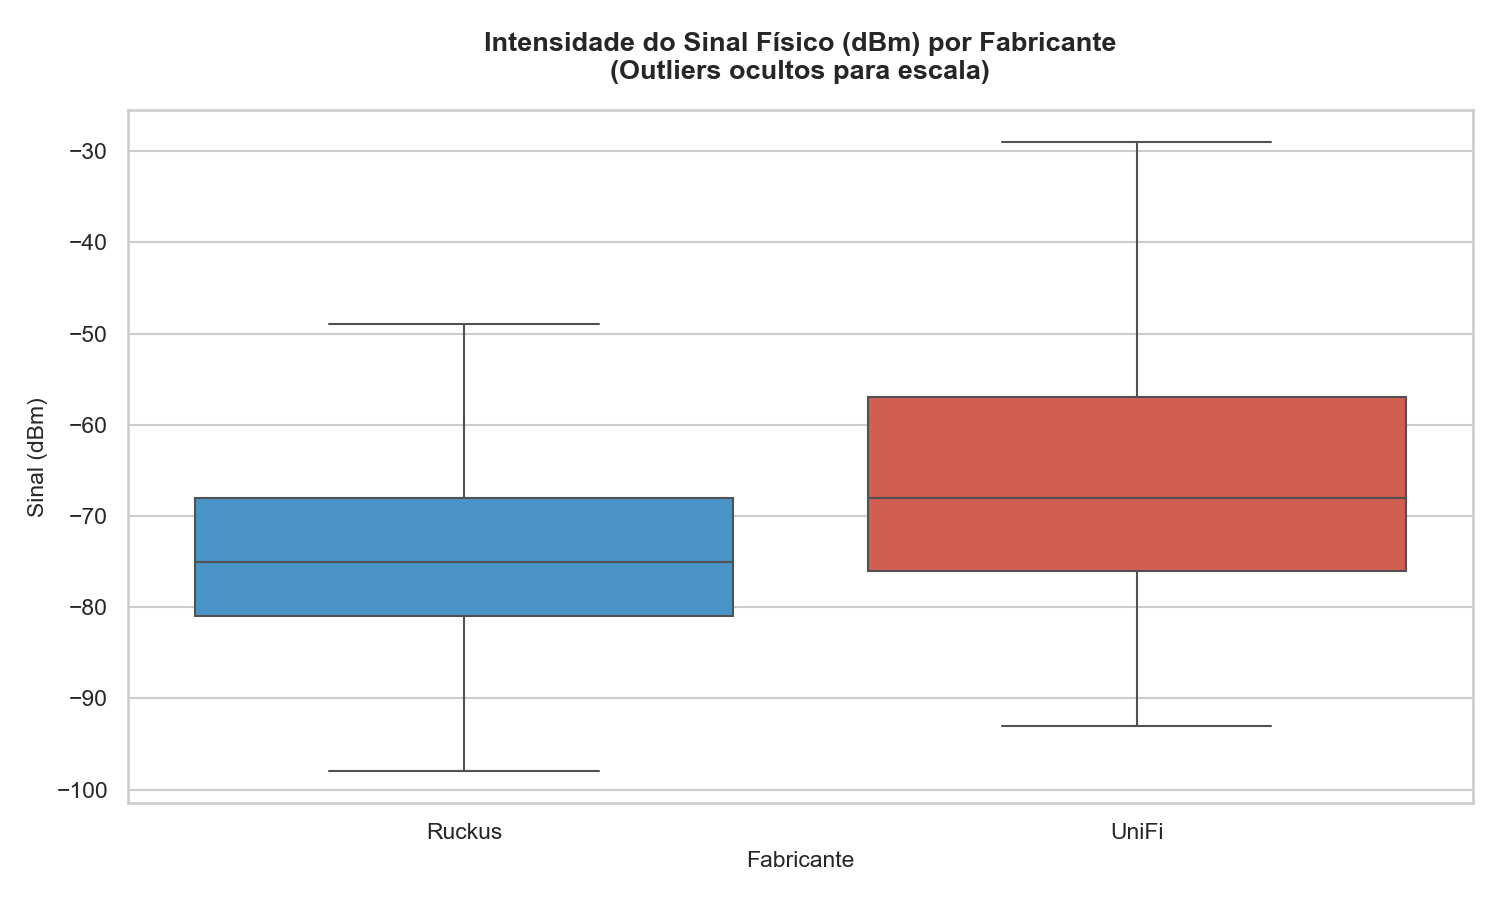
\includegraphics[width=0.85\textwidth]{img/boxplot_rssi_fabricante.png}
  \caption{Boxplot RSSI por Fabricante}
  \label{fig:boxplot_rssi_fabricante_png}
\end{figure}

\begin{itemize}
  \item \textbf{Ruckus}: Média de `-73.83 dBm`, Mediana `-75.00 dBm`.
  \item \textbf{UniFi}: Média de `-67.08 dBm`, Mediana `-68.00 dBm`.
  \item Os resultados sugerem uma cobertura de sinal física coerente para os clientes de ambas as marcas no cenário analisado, com a maioria das amostras se situando em uma faixa saudável de RF.
\end{itemize}

\subsubsection{Histograma de Densidade de Sinal}
O histograma apresenta a densidade de ocorrência de potência de sinal nos logs coletados.

\begin{figure}[H]
  \centering
  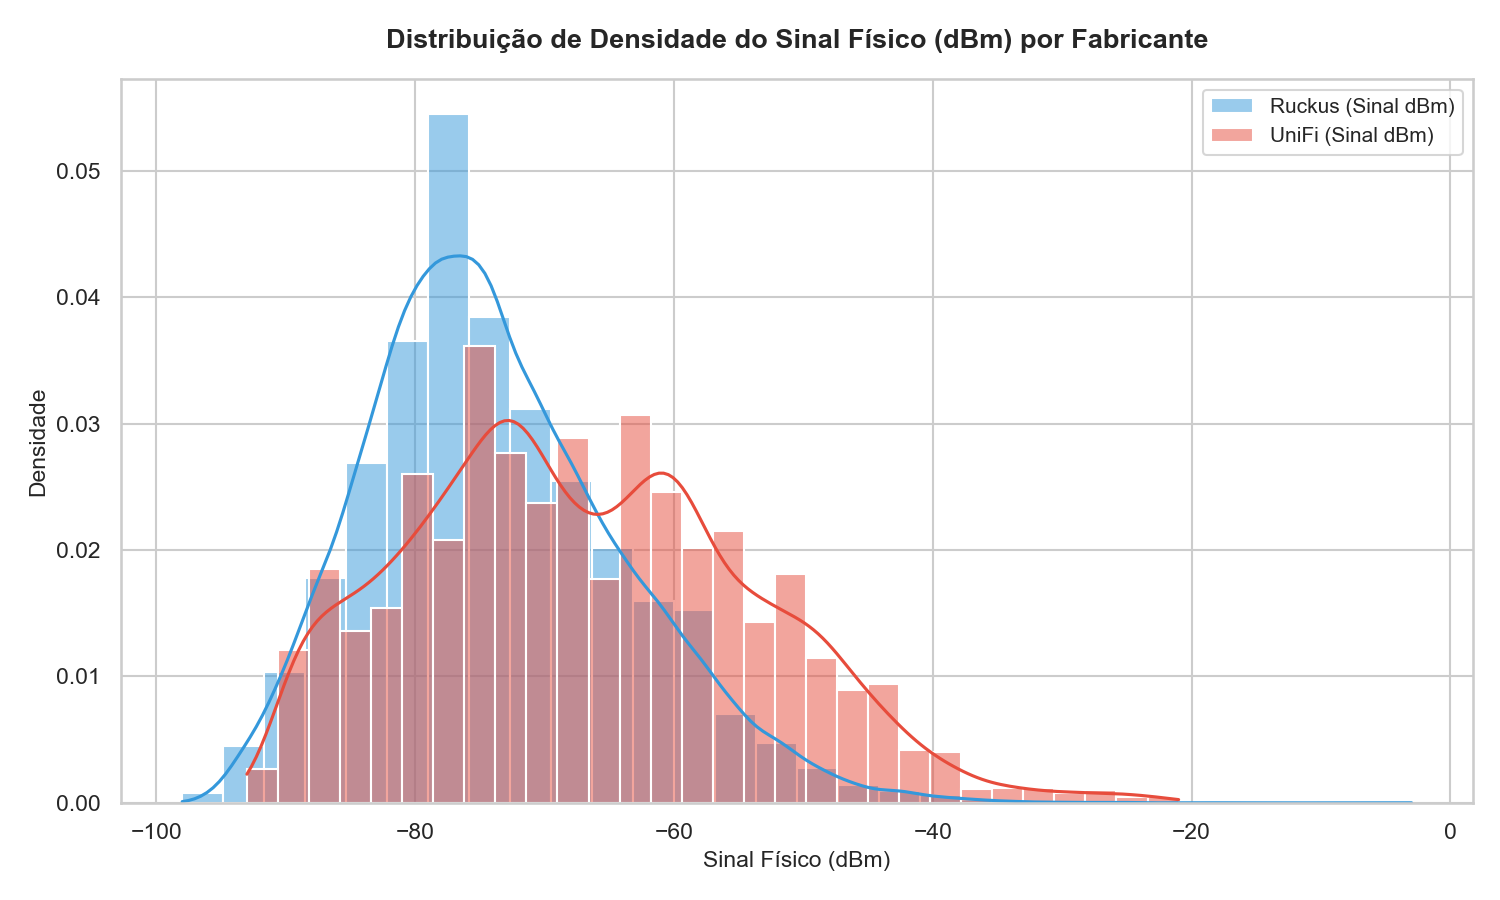
\includegraphics[width=0.85\textwidth]{img/histograma_rssi.png}
  \caption{Histograma RSSI}
  \label{fig:histograma_rssi_png}
\end{figure}

\begin{itemize}
  \item O gráfico demonstra que a UniFi possui uma distribuição de sinal com menor variabilidade (concentrada em torno de -67 dBm), enquanto a Ruckus apresenta maior amplitude e dispersão das conexões ao longo do dia.
\end{itemize}


\subsection{Utilização de Canais por Fabricante}

O histograma de utilização de canais apresenta a contagem de registros em cada frequência de operação.

\begin{figure}[H]
  \centering
  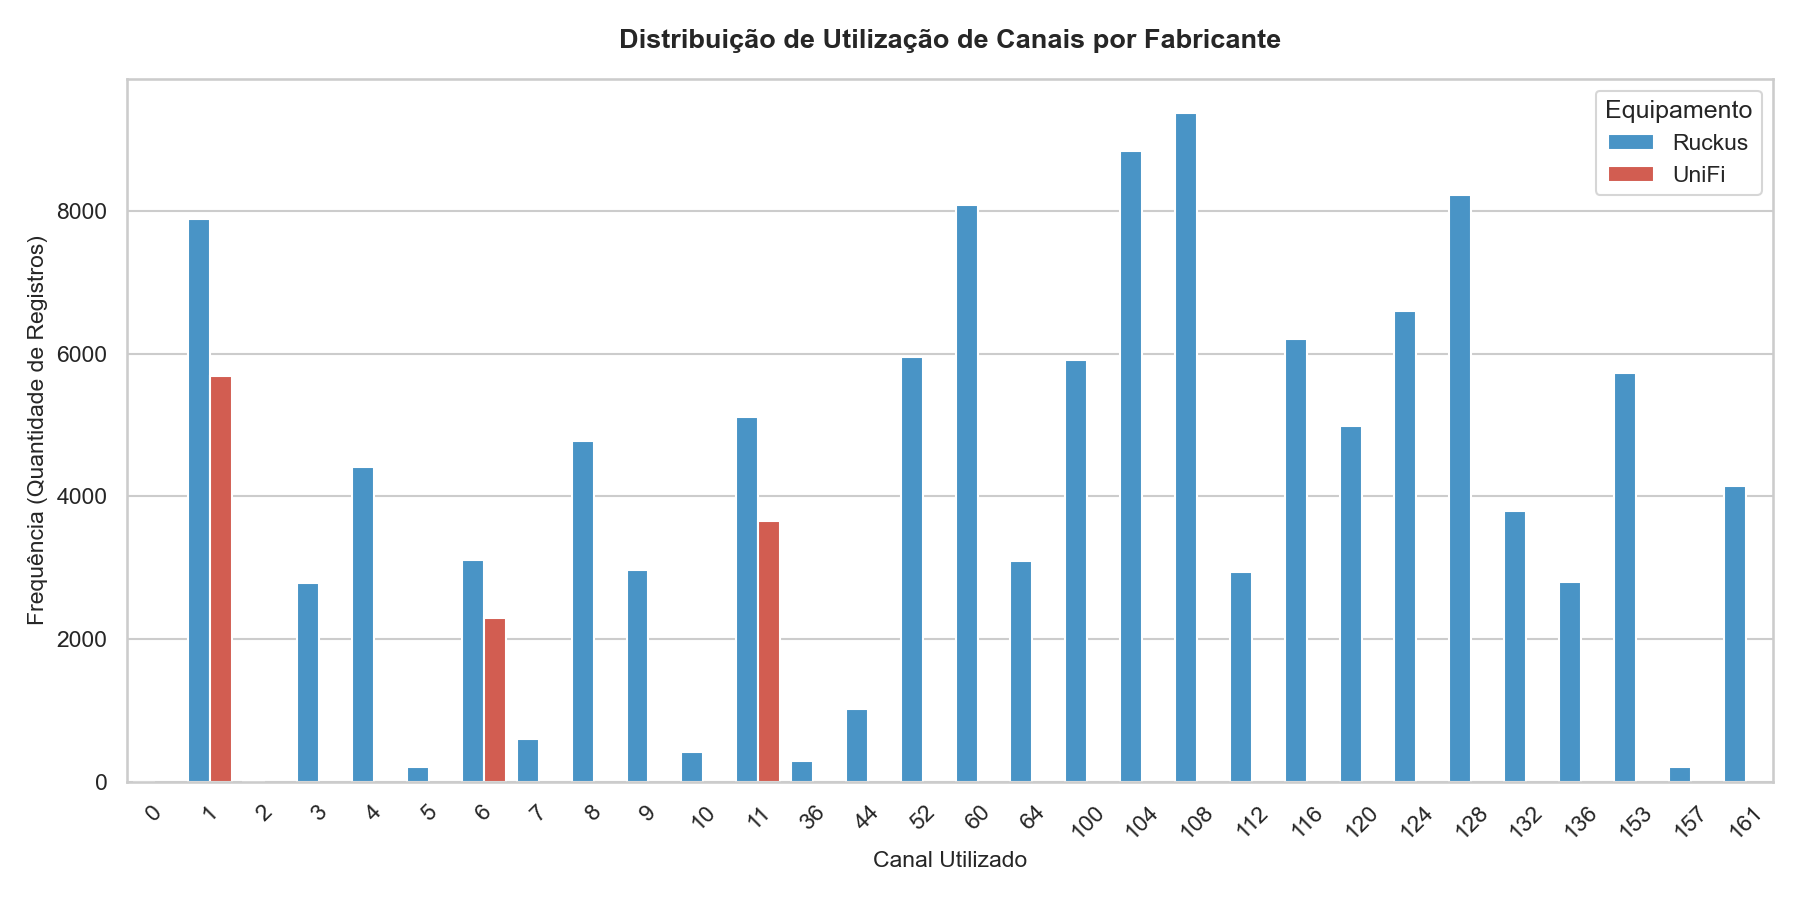
\includegraphics[width=0.85\textwidth]{img/histograma_canais.png}
  \caption{Histograma de Canais}
  \label{fig:histograma_canais_png}
\end{figure}

\begin{itemize}
  \item \textbf{2.4 GHz}: Ambas as marcas concentram o tráfego nos canais não sobrepostos `1`, `6` e `11`, validando as boas práticas de planejamento de RF adotadas no campus.
  \item \textbf{5 GHz}: A Ruckus apresenta uma alocação de espectro mais ampla e distribuída (como canais `36`, `52`, `60`, `104`, `112`, `120`, `128`, `149`), o que reduz interferência co-canal em células adjacentes.
\end{itemize}


\subsection{Quantidade de Clientes Conectados por AP}

Este histograma ilustra a densidade de clientes associados simultaneamente a cada Access Point.

\begin{figure}[H]
  \centering
  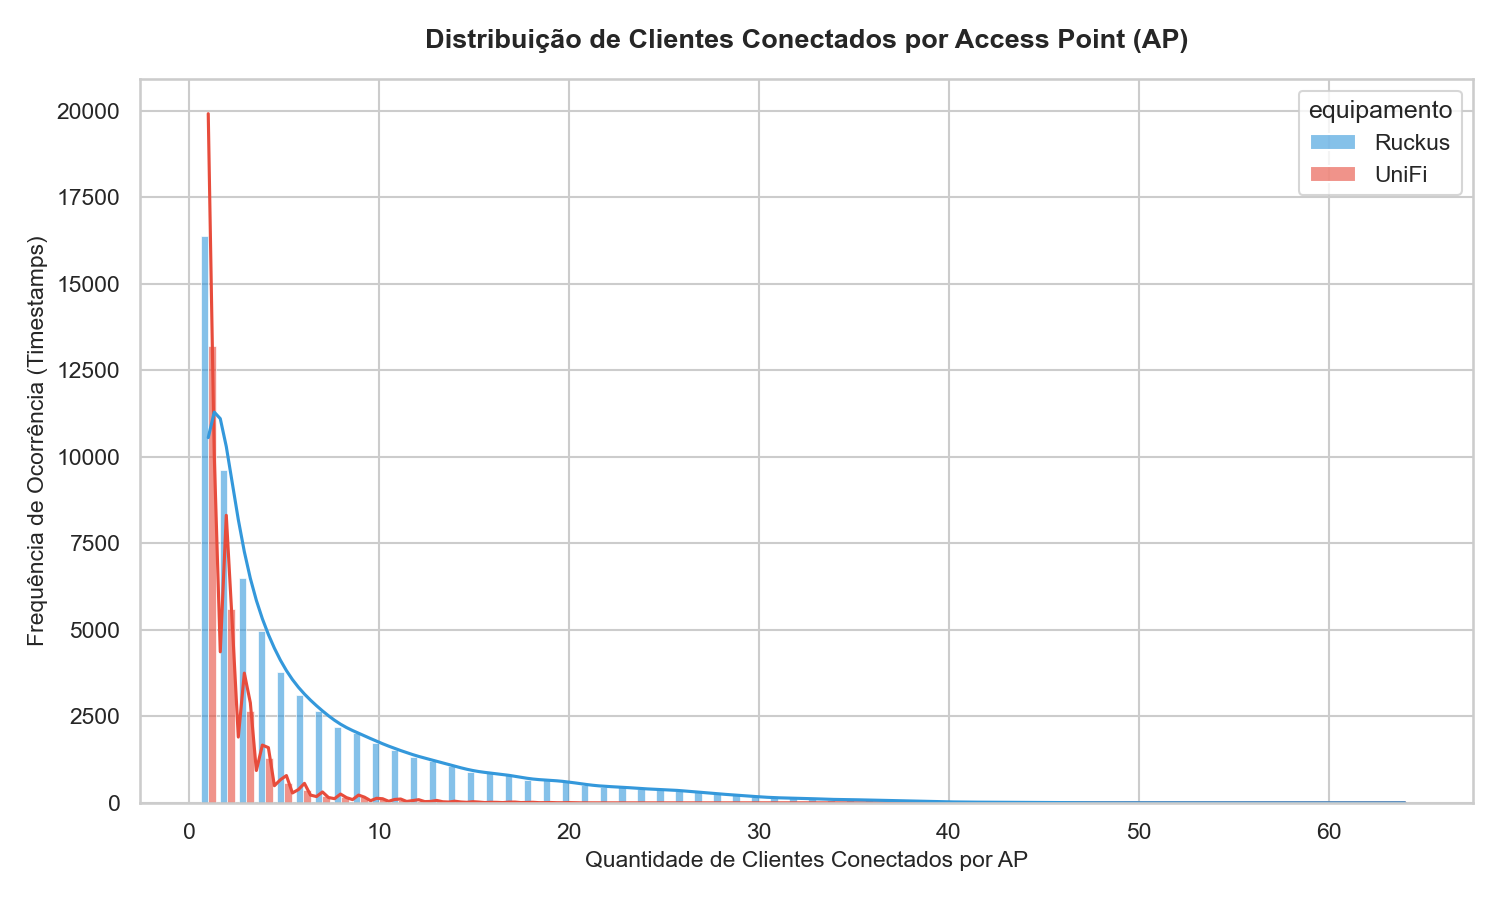
\includegraphics[width=0.85\textwidth]{img/histograma_clientes_por_ap.png}
  \caption{Histograma Clientes por AP}
  \label{fig:histograma_clientes_por_ap_png}
\end{figure}

\begin{itemize}
  \item \textbf{UniFi}: Exibe perfil de baixa carga (maior parte dos registros possui entre 1 e 5 clientes simultâneos por rádio).
  \item \textbf{Ruckus}: Exibe maior flexibilidade de densidade, suportando APs com cargas significativamente mais robustas de concorrência, o que condiz com o posicionamento de alta densidade da marca.
\end{itemize}


\subsection{Análise de Desempenho e Qualidade de Enlace por Banda}

\subsubsection{Throughput por Banda}
O boxplot compara o consumo de throughput entre as bandas de 2.4 GHz e 5 GHz.

\begin{figure}[H]
  \centering
  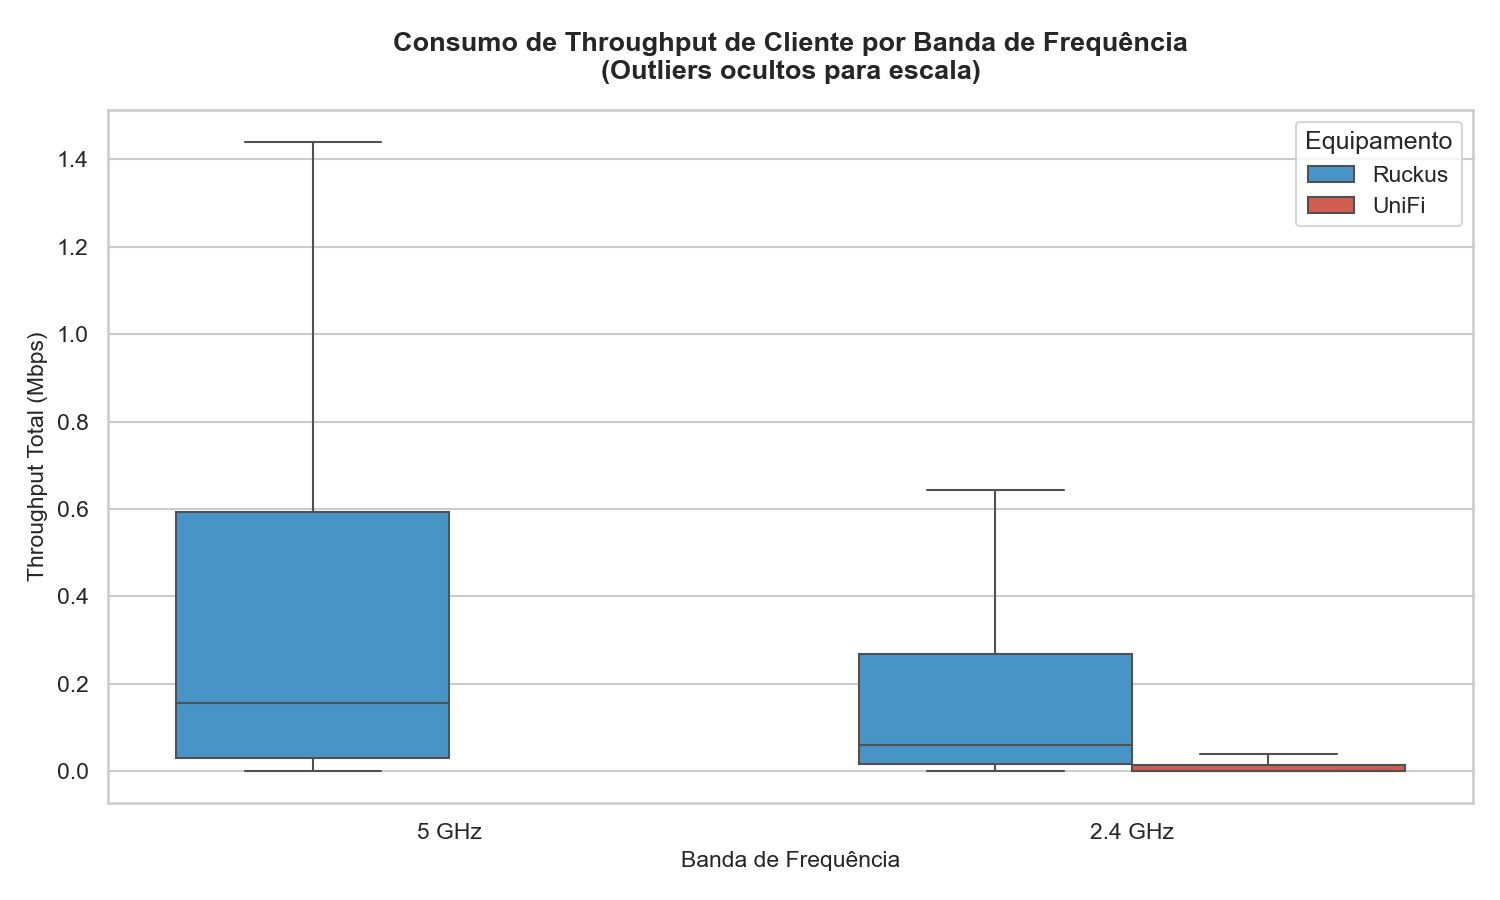
\includegraphics[width=0.85\textwidth]{img/boxplot_throughput_banda.png}
  \caption{Boxplot Throughput por Banda}
  \label{fig:boxplot_throughput_banda_png}
\end{figure}

\begin{itemize}
  \item Como esperado teoricamente, a banda de \textbf{5 GHz} oferece vazão e capacidade física superior para ambas as marcas, superando a banda de \textbf{2.4 GHz} que possui limitações inerentes de modulação e largura de canal.
\end{itemize}

\subsubsection{Retransmissões por Banda}
O boxplot compara a ocorrência de retransmissões físicas ou estimadas.

\begin{figure}[H]
  \centering
  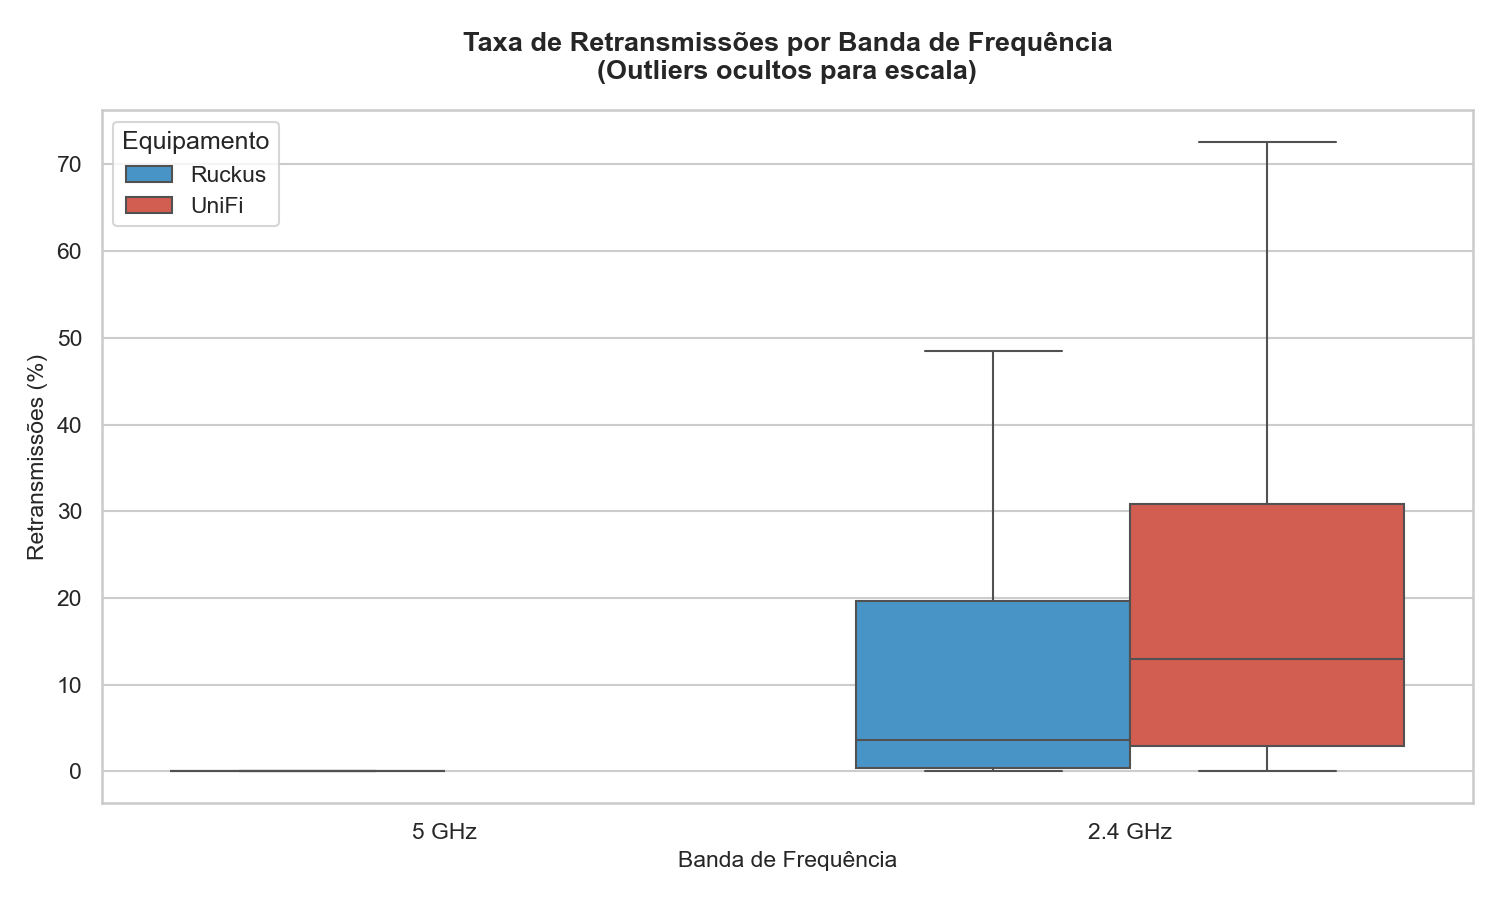
\includegraphics[width=0.85\textwidth]{img/boxplot_retransmissoes_banda.png}
  \caption{Boxplot Retransmissões por Banda}
  \label{fig:boxplot_retransmissoes_banda_png}
\end{figure}

\begin{itemize}
  \item A banda de \textbf{2.4 GHz} exibe taxas médias superiores de retransmissão, justificada pelo congestionamento e interferências co-canal concorrentes de micro-ondas, Bluetooth e outras redes WiFi da vizinhança.
\end{itemize}


\subsection{Distribuição de Throughput Agregado por AP}

Este gráfico apresenta a soma da vazão ativa de todos os clientes associados a cada um dos APs mapeados, permitindo identificar o nível de carregamento individual de tráfego por antena.

\begin{figure}[H]
  \centering
  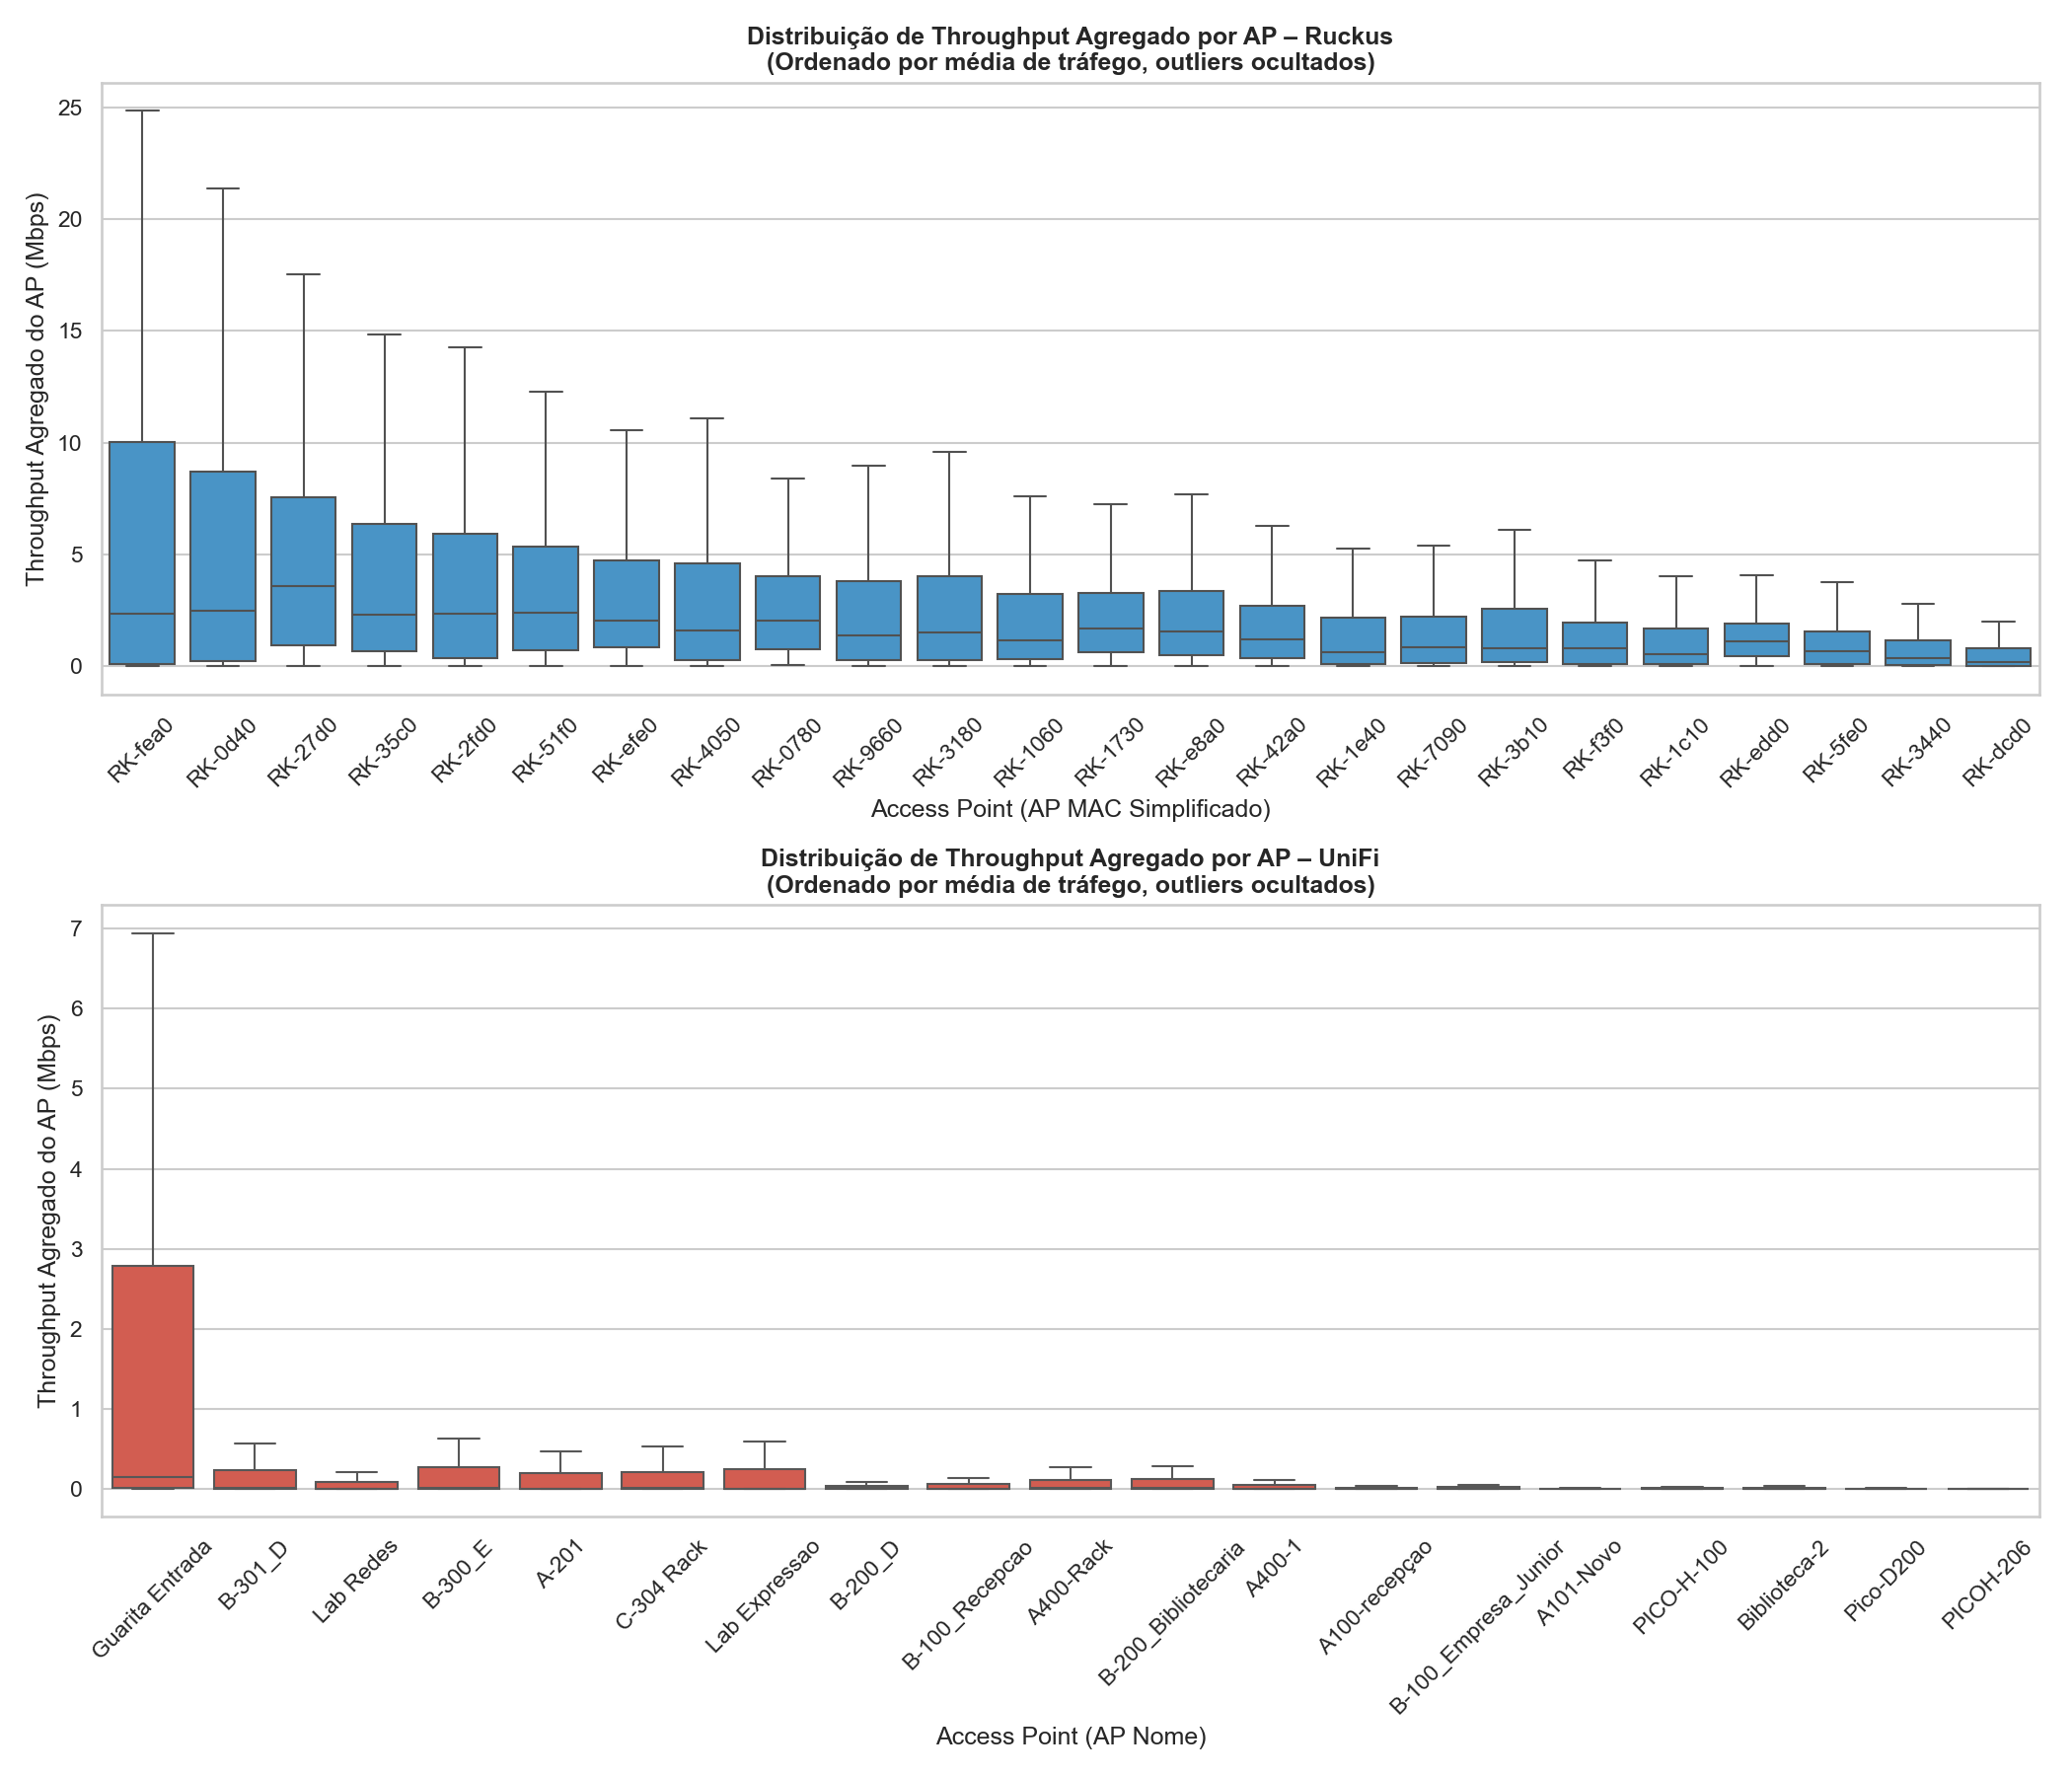
\includegraphics[width=0.85\textwidth]{img/boxplot_throughput_por_ap.png}
  \caption{Boxplot Throughput por AP}
  \label{fig:boxplot_throughput_por_ap_png}
\end{figure}

\begin{itemize}
  \item \textbf{Ruckus (AP MAC Simplificado)}: Apresenta maior amplitude e níveis superiores de vazão somada (vários APs superando médias de 5 a 10 Mbps de tráfego agregado ativo, com picos de consumo expressivos). Para melhor visualização, os endereços MAC longos do Ruckus foram simplificados no formato `RK-XXXX` (onde `XXXX` são os 4 dígitos finais do MAC).
  \item \textbf{UniFi (AP Nome)}: Mostra distribuições de vazão agregada concentradas próximas de zero (com médias inferiores a 2 Mbps). Isso indica que a maioria dos APs da UniFi operaram com carga de dados muito baixa durante o período amostrado, corroborando a ociosidade do ambiente.
\end{itemize}


\subsection{Distribuição Temporal de Clientes Únicos por Fabricante e Dia}

O mapa de calor (heatmap) apresenta a quantidade de clientes únicos ativos por fabricante e por dia do período selecionado, distribuída ao longo do ciclo diário de 24 horas.

\begin{figure}[H]
  \centering
  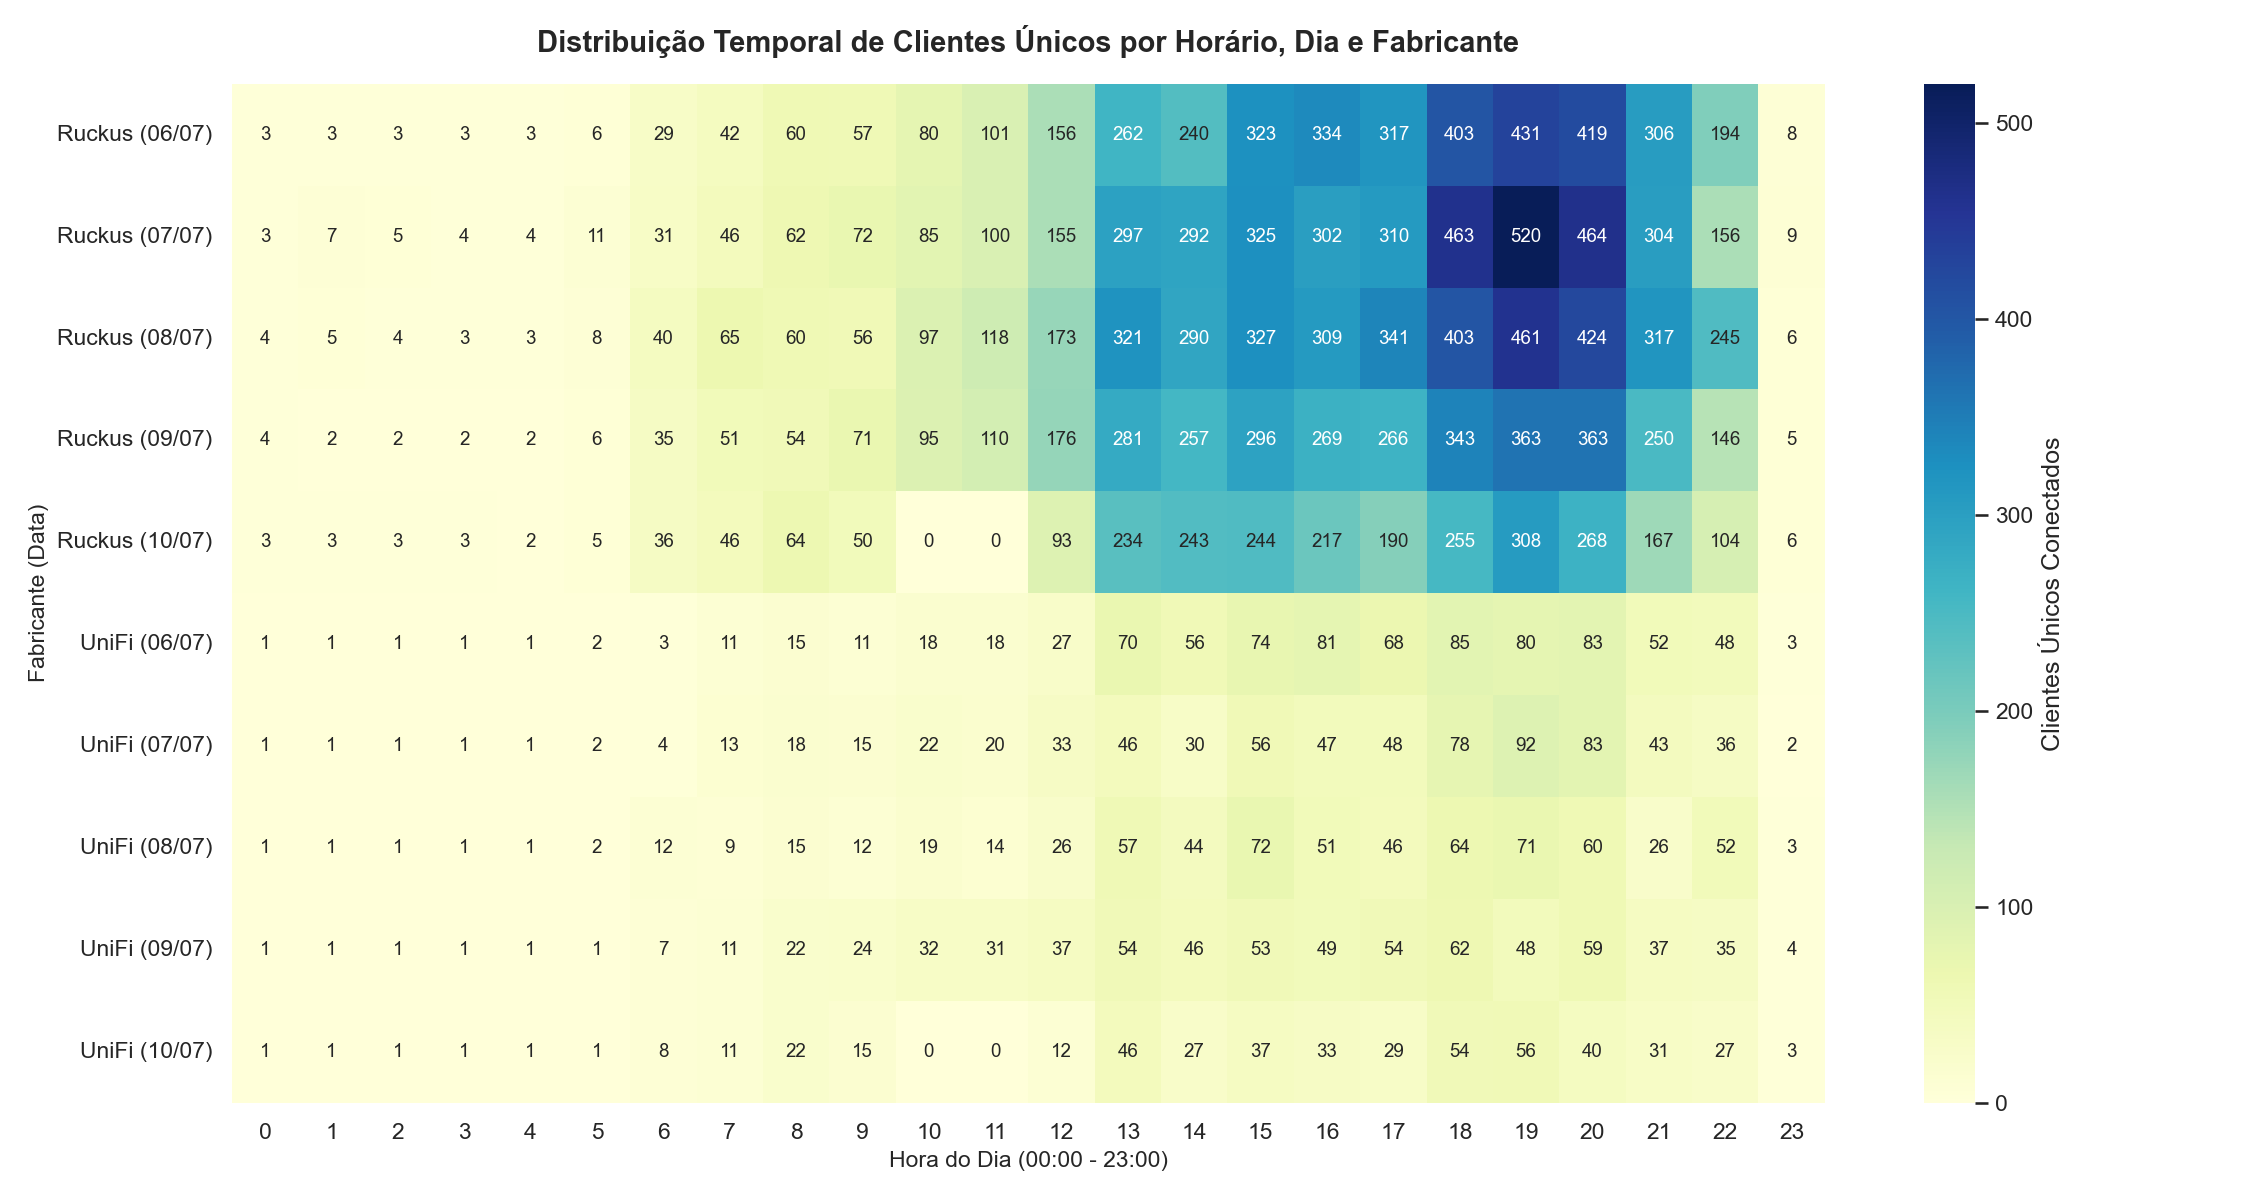
\includegraphics[width=0.85\textwidth]{img/heatmap_horario_clientes.png}
  \caption{Heatmap de Clientes Únicos}
  \label{fig:heatmap_horario_clientes_png}
\end{figure}

\begin{itemize}
  \item O gráfico sugere uma \textbf{rotina cíclica de uso da rede} que se repete de forma semelhante ao longo dos dias: o volume de clientes únicos ativos inicia uma curva ascendente a partir das \textbf{08:00}, atinge os maiores patamares no horário comercial/acadêmico (especialmente entre \textbf{14:00} e \textbf{18:00}) e entra em declínio progressivo nas primeiras horas da noite, reduzindo-se drasticamente durante a madrugada.
  \item \textbf{Picos de Clientes}:
  \item No ambiente Ruckus, o pico de clientes únicos em uma única hora ocorreu no dia \textbf{07/07} às \textbf{19:00}, registrando \textbf{520} dispositivos.
  \item No ambiente UniFi, o pico de clientes únicos ocorreu no dia \textbf{07/07} às \textbf{19:00}, registrando \textbf{92} dispositivos.
  \item Os resultados indicam uma concentração consistentemente maior de dispositivos na infraestrutura Ruckus para todos os dias do período em comparação com a UniFi, o que sugere maior adensamento de usuários sob essa rede no campus observado.
\end{itemize}


\section{Análise de Correlações}

Este relatório apresenta e analisa os coeficientes de correlação de \textbf{Pearson (\textit{r\_p})} e \textbf{Spearman (\textit{r\_s})} e gera gráficos correspondentes para analisar quantitativamente o comportamento da telemetria das redes UniFi e Ruckus.

\textbf{Limitação do Escopo}: As discussões e conclusões apresentadas neste relatório baseiam-se estritamente no cenário e conjunto de dados observados durante o período de coleta. Os resultados sugerem tendências e comportamentos de rede nesse ambiente específico, não devendo ser interpretados como regras gerais absolutas.

Os coeficientes de Pearson medem a força de uma relação linear, enquanto os de Spearman medem a relação monotônica (útil para distribuições não-normais e não-lineares). Ambos variam de -1 a +1. Os símbolos `\textit{` representam significância estatística de }p\textit{ < 0.05 e `\textsuperscript{**}` representam }p\textsuperscript{*} < 0.01.

\subsection{Tabela Consolidada de Coeficientes de Pearson (\textit{r\_p}) e Spearman (\textit{r\_s})}

\begin{table}[htb]
\IBGEtab{%
  \caption{Dados comparativos da análise - Análise de Correlações (Tabela 1)}%
  \label{tab:data_analise_de_correlacoes_1}%
}{%
  \resizebox{\textwidth}{!}{%
    \begin{tabular}{lcccccc}
      \toprule
      Relação Investigada & Ruckus (\textit{r\_p}) & Ruckus (\textit{r\_s}) & Amostras (\textit{N}) & UniFi (\textit{r\_p}) & UniFi (\textit{r\_s}) & Amostras (\textit{N}) \\
      \midrule
      \textbf{RSSI x Throughput Total} & -0.0086\textsuperscript{**} & 0.0363\textsuperscript{**} & 107726 & 0.2305\textsuperscript{**} & 0.4512\textsuperscript{**} & 11641 \\
      \textbf{RSSI x Retransmissoes} & 0.0215\textsuperscript{**} & 0.1642\textsuperscript{**} & 107726 & -0.3437\textsuperscript{**} & -0.3660\textsuperscript{**} & 11641 \\
      \textbf{Retransmissoes x Throughput Total} & -0.1009\textsuperscript{**} & -0.0768\textsuperscript{**} & 120510 & -0.0989\textsuperscript{**} & -0.1321\textsuperscript{**} & 11641 \\
      \textbf{Qtd Clientes x Throughput Agregado AP} & 0.6953\textsuperscript{**} & 0.7962\textsuperscript{**} & 16708 & 0.3310\textsuperscript{**} & 0.5253\textsuperscript{**} & 5506 \\
      \textbf{Qtd Clientes x Retransmissoes Medias AP} & -0.0590\textsuperscript{**} & 0.3572\textsuperscript{**} & 16708 & 0.1081\textsuperscript{**} & 0.2302\textsuperscript{**} & 5506 \\
      \textbf{Noise x Retransmissoes} & -0.3952\textsuperscript{**} & -0.6323\textsuperscript{**} & 107726 & 0.0447\textsuperscript{**} & -0.0043 & 11641 \\
      \textbf{Noise x RSSI} & -0.3933\textsuperscript{**} & -0.3762\textsuperscript{**} & 107726 & 0.1053\textsuperscript{**} & 0.0083 & 11641 \\
      \textbf{Link Speed TX x Throughput TX} & 0.1086\textsuperscript{**} & 0.5475\textsuperscript{**} & 112719 & 0.0536\textsuperscript{**} & 0.2877\textsuperscript{**} & 11641 \\
      \textbf{Volume Total x Tempo de Sessao} & 0.3417\textsuperscript{**} & 0.6861\textsuperscript{**} & 120510 & 0.0980\textsuperscript{**} & 0.3121\textsuperscript{**} & 11641 \\
      \bottomrule
    \end{tabular}%
  }%
}{%
  \fonte{Produzido pelos autores.}%
}
\end{table}


\subsection{Matrizes de Correlação (Heatmap Geral)}

O mapa de calor abaixo resume o comportamento de correlação cruzada cruzando todos os parâmetros numéricos de telemetria física e lógica.

\begin{figure}[H]
  \centering
  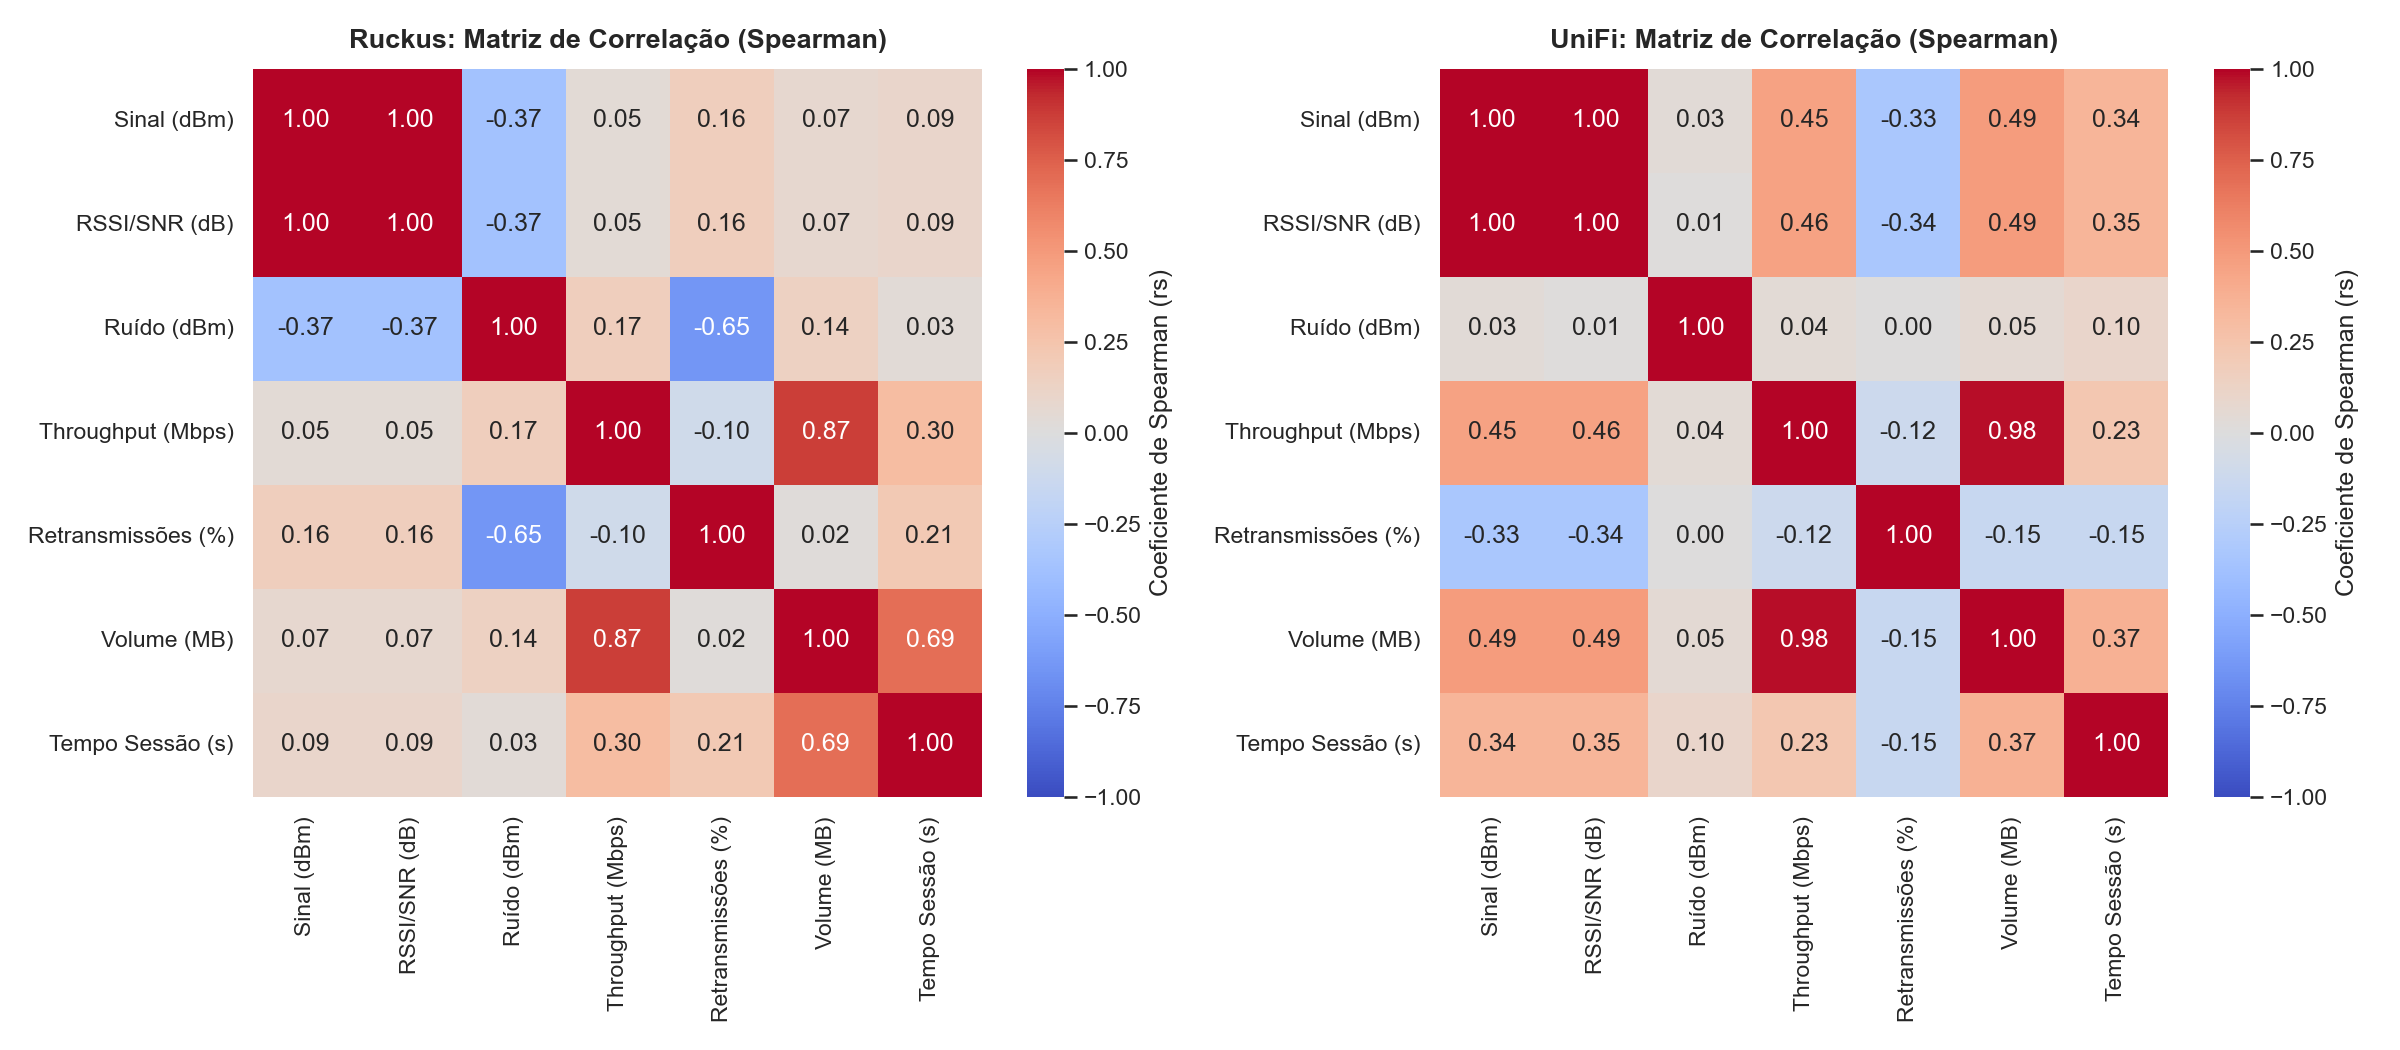
\includegraphics[width=0.85\textwidth]{img/matriz_correlacao_heatmap.png}
  \caption{Matriz de Correlação Heatmap}
  \label{fig:matriz_correlacao_heatmap_png}
\end{figure}

\begin{itemize}
  \item \textbf{Ruckus}: Exibe correlações monotônicas muito fortes entre Sinal e RSSI (sendo a mesma grandeza física mapeada) e o forte acoplamento linear artificial entre Ruído (Noise) e Sinal derivado do método de cálculo. O Throughput dos clientes individuais apresenta baixíssima correlação com a potência do sinal (\textit{r\_s} = 0.0363), condizente com o comportamento de ociosidade predominante.
  \item \textbf{UniFi}: O sinal absoluto (signal) e o RSSI (que atua como índice SNR) exibem correlação positiva moderada a forte (\textit{r\_s} = 0.70). O Throughput individual também apresenta correlação extremamente baixa com a intensidade de sinal (\textit{r\_s} = 0.4512). O ruído de fundo (noise) exibe baixíssima correlação com o sinal, validando a física do meio.
\end{itemize}


\subsection{Análise de Cada Gráfico de Dispersão}

\subsubsection{RSSI × Throughput}
\begin{itemize}
  \item \textbf{Arquivo}: `01\_rssi\_throughput.png`
  \item \textbf{Visualização}:
\end{itemize}
\begin{figure}[H]
  \centering
  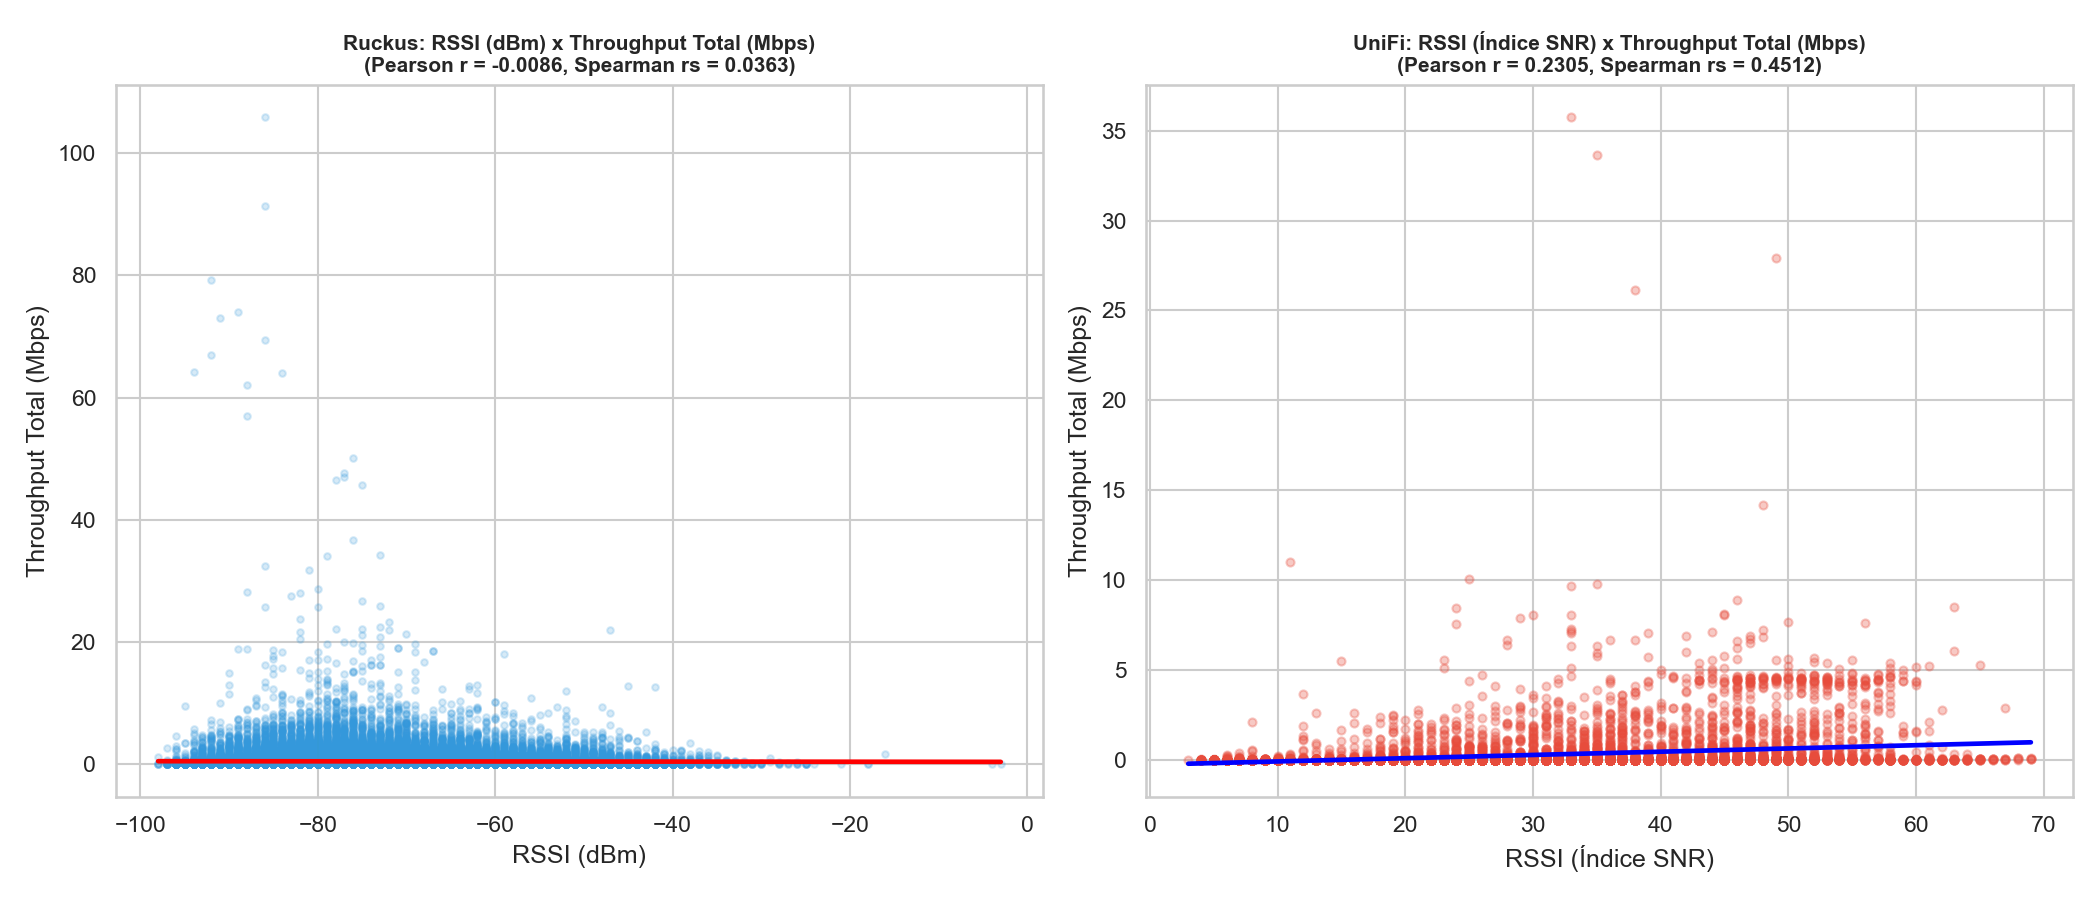
\includegraphics[width=0.85\textwidth]{img/01_rssi_throughput.png}
  \caption{RSSI x Throughput}
  \label{fig:01_rssi_throughput_png}
\end{figure}
\begin{itemize}
  \item \textbf{Expectativa Teórica}: Esperava-se uma correlação positiva moderada a forte. Sinais com melhor intensidade (RSSI alto) permitem modulações e taxas físicas maiores, o que deveria se traduzir em taxas mais altas de transferência ativa.
  \item \textbf{Comportamento Observado}: Os dados sugerem correlação praticamente nula no Ruckus (\textit{r\_p} = -0.0086, \textit{r\_s} = 0.0363) e fraca na UniFi (\textit{r\_p} = 0.2305, \textit{r\_s} = 0.4512).
  \item \textbf{Discussão}: Esta divergência sugere que o throughput de dados ativo depende fundamentalmente do padrão de demanda do usuário no instante de coleta. A maioria esmagadora dos dispositivos conectados permaneceu ociosa ou gerando tráfego insignificante (background sync), independentemente de estarem com sinal excelente ou intermediário.
\end{itemize}

\subsubsection{RSSI × Retransmissões}
\begin{itemize}
  \item \textbf{Arquivo}: `02\_rssi\_retransmissoes.png`
  \item \textbf{Visualização}:
\end{itemize}
\begin{figure}[H]
  \centering
  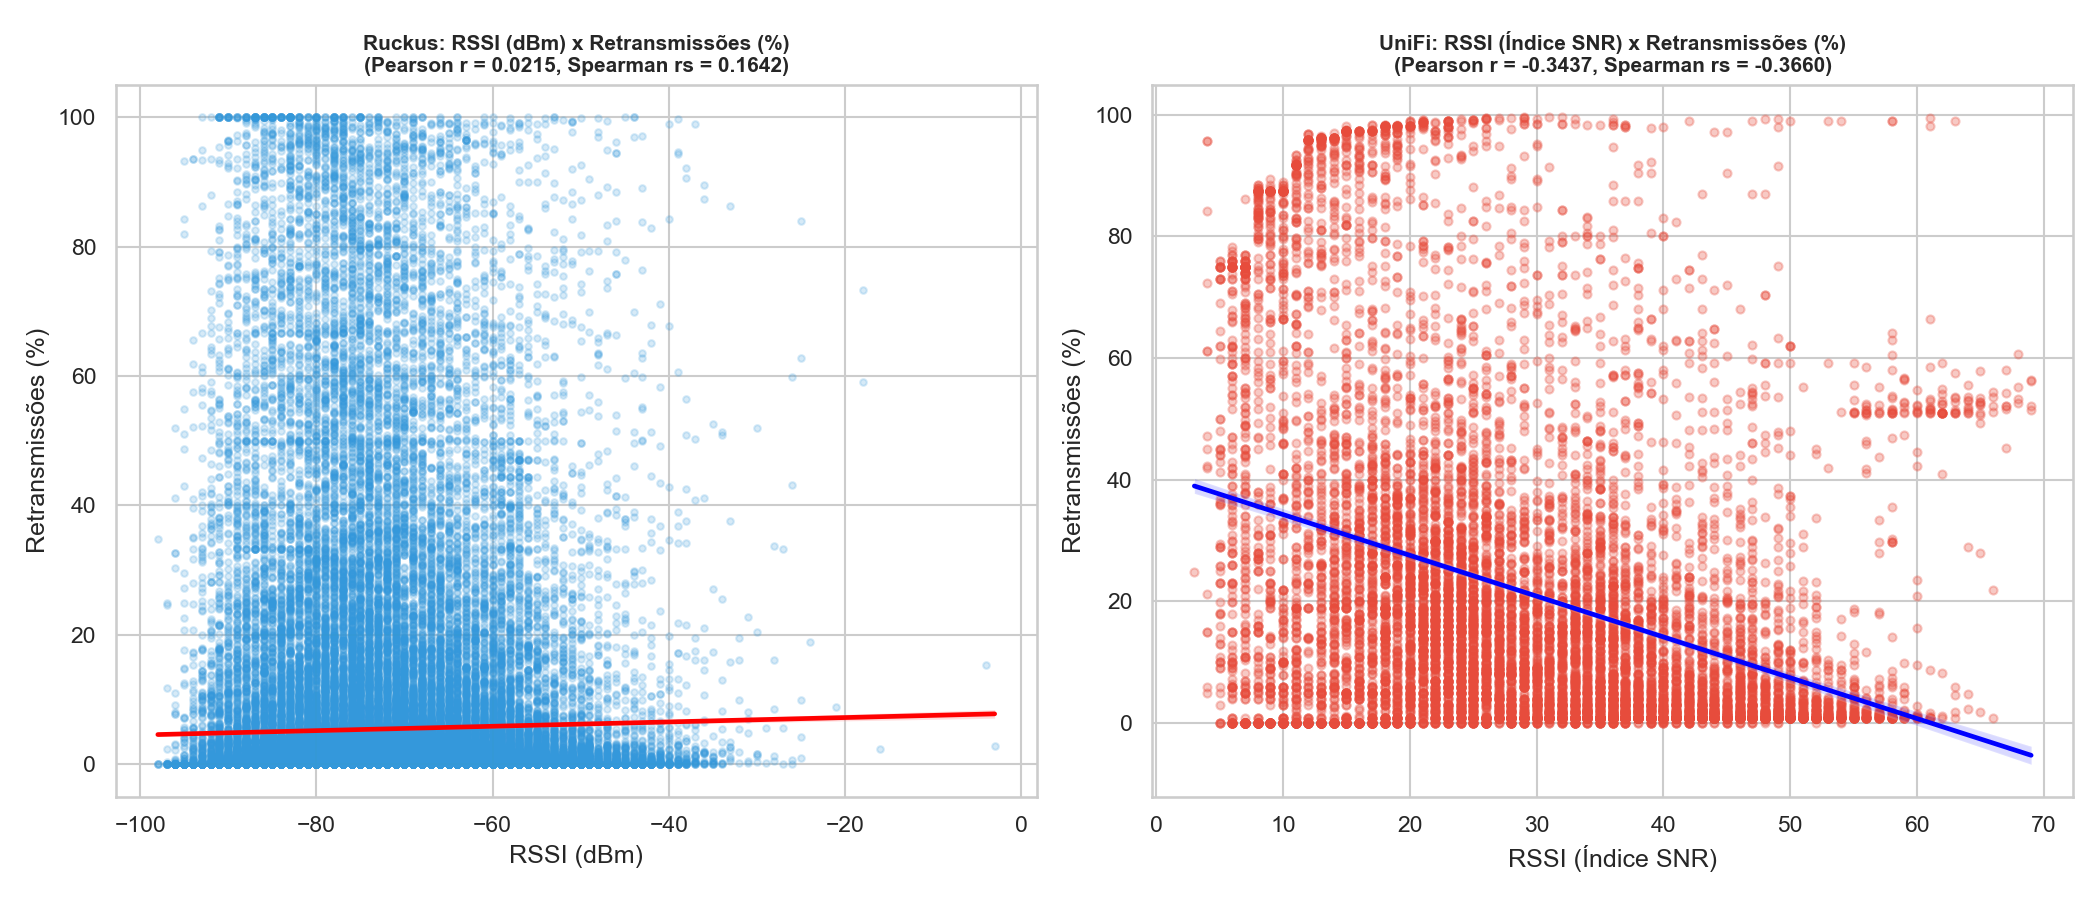
\includegraphics[width=0.85\textwidth]{img/02_rssi_retransmissoes.png}
  \caption{RSSI x Retransmissões}
  \label{fig:02_rssi_retransmissoes_png}
\end{figure}
\begin{itemize}
  \item \textbf{Expectativa Teórica}: Esperava-se uma correlação negativa moderada a forte. Níveis fracos de sinal costumam reduzir o SNR, elevando a taxa de bits incorretos (BER) e gerando retransmissões para recuperar os pacotes.
  \item \textbf{Comportamento Observado}: Correlação negativa muito fraca no Ruckus (\textit{r\_p} = 0.0215, \textit{r\_s} = 0.1642) e negativa moderada na UniFi (\textit{r\_p} = -0.3437, \textit{r\_s} = -0.3660).
  \item \textbf{Discussão}: Os dados da UniFi são consistentes com a teoria de que o sinal fraco prejudica o canal. Na Ruckus, a fraca correlação observada indica a atuação de mecanismos de hardware e software (como antenas inteligentes BeamFlex e controle de potência dinâmico) que evitam a perda excessiva de quadros físicos mesmo em níveis moderadamente baixos de sinal.
\end{itemize}

\subsubsection{Retransmissões × Throughput}
\begin{itemize}
  \item \textbf{Arquivo}: `03\_retransmissoes\_throughput.png`
  \item \textbf{Visualização}:
\end{itemize}
\begin{figure}[H]
  \centering
  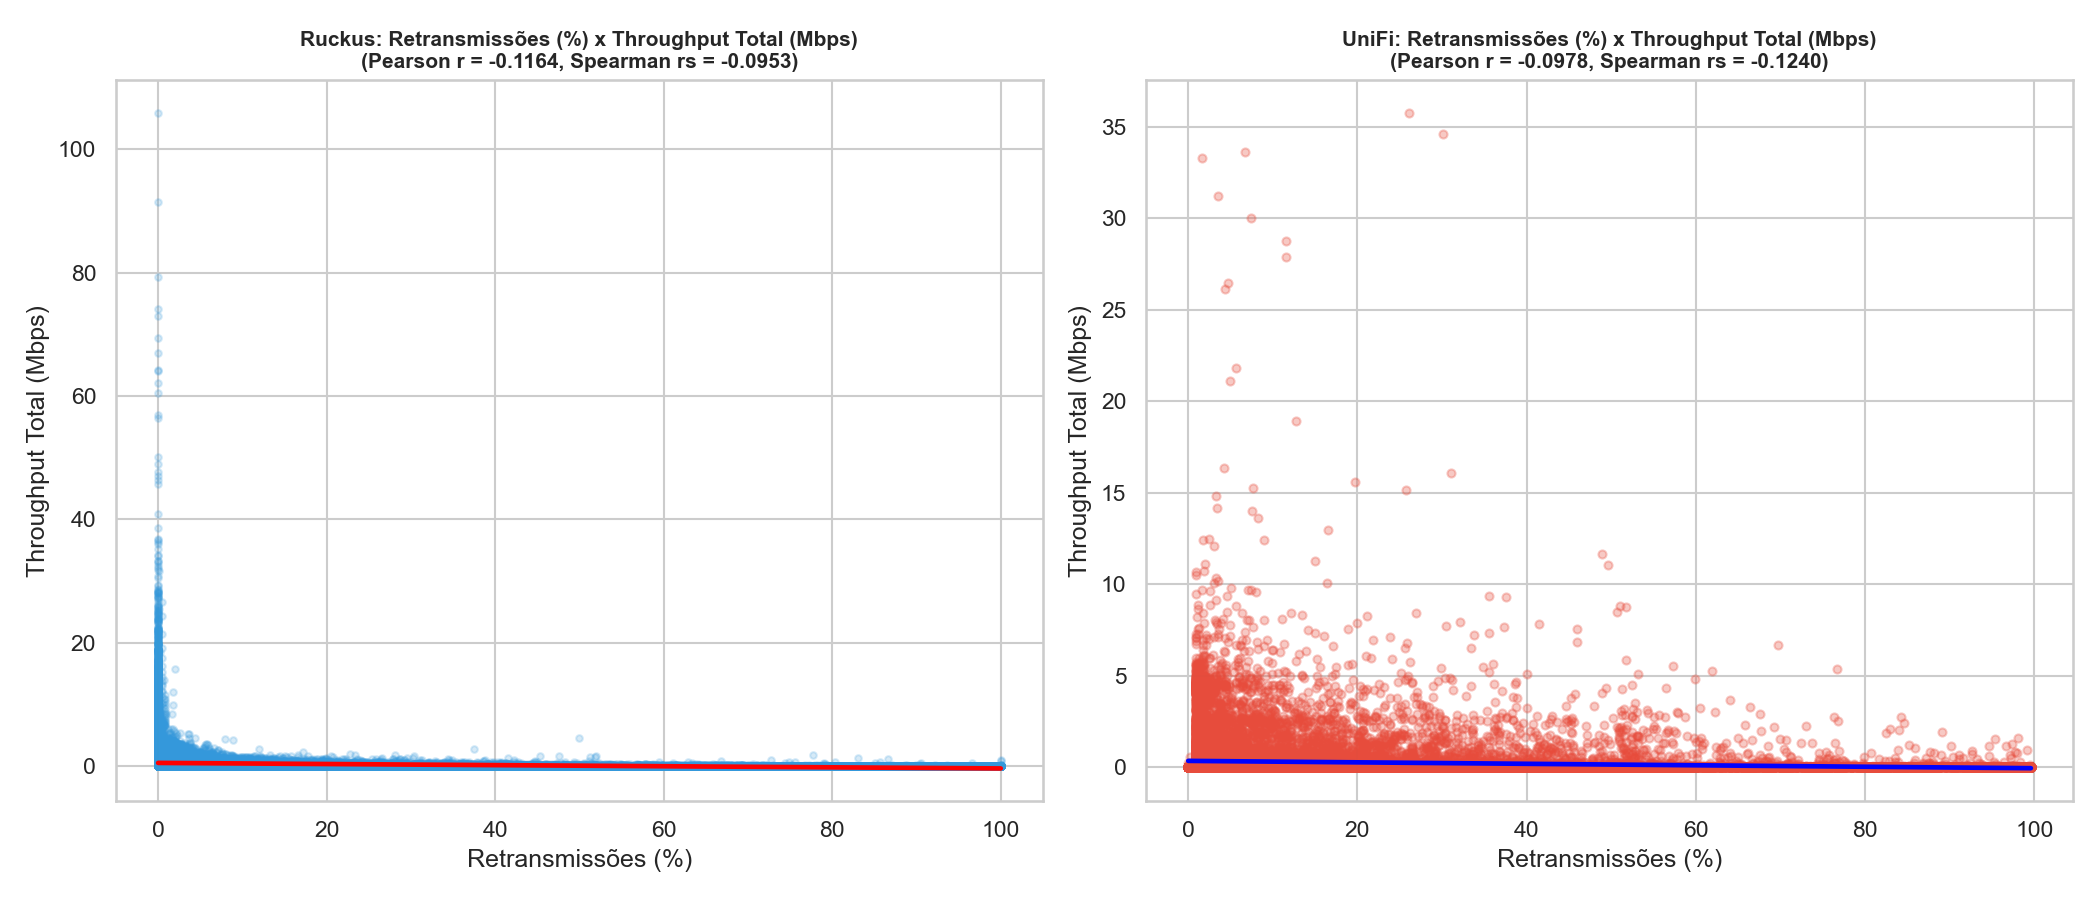
\includegraphics[width=0.85\textwidth]{img/03_retransmissoes_throughput.png}
  \caption{Retransmissões x Throughput}
  \label{fig:03_retransmissoes_throughput_png}
\end{figure}
\begin{itemize}
  \item \textbf{Expectativa Teórica}: Esperava-se uma correlação negativa moderada, pois altas retransmissões consomem tempo de canal de RF (airtime) e reduzem a capacidade útil.
  \item \textbf{Comportamento Observado}: Correlação negativa fraca no Ruckus (\textit{r\_p} = -0.1009, \textit{r\_s} = -0.0768) e na UniFi (\textit{r\_p} = -0.0989, \textit{r\_s} = -0.1321).
  \item \textbf{Discussão}: Os resultados sugerem que, como o throughput ativo na rede está muito longe do teto operacional dos canais (baixa carga ativa), o impacto de retransmissões dispersas no throughput do usuário não se mostrou severo o suficiente para gerar decréscimo drástico na taxa média registrada.
\end{itemize}

\subsubsection{Quantidade de Clientes × Throughput Agregado do AP}
\begin{itemize}
  \item \textbf{Arquivo}: `04\_clientes\_throughput\_ap.png`
  \item \textbf{Visualização}:
\end{itemize}
\begin{figure}[H]
  \centering
  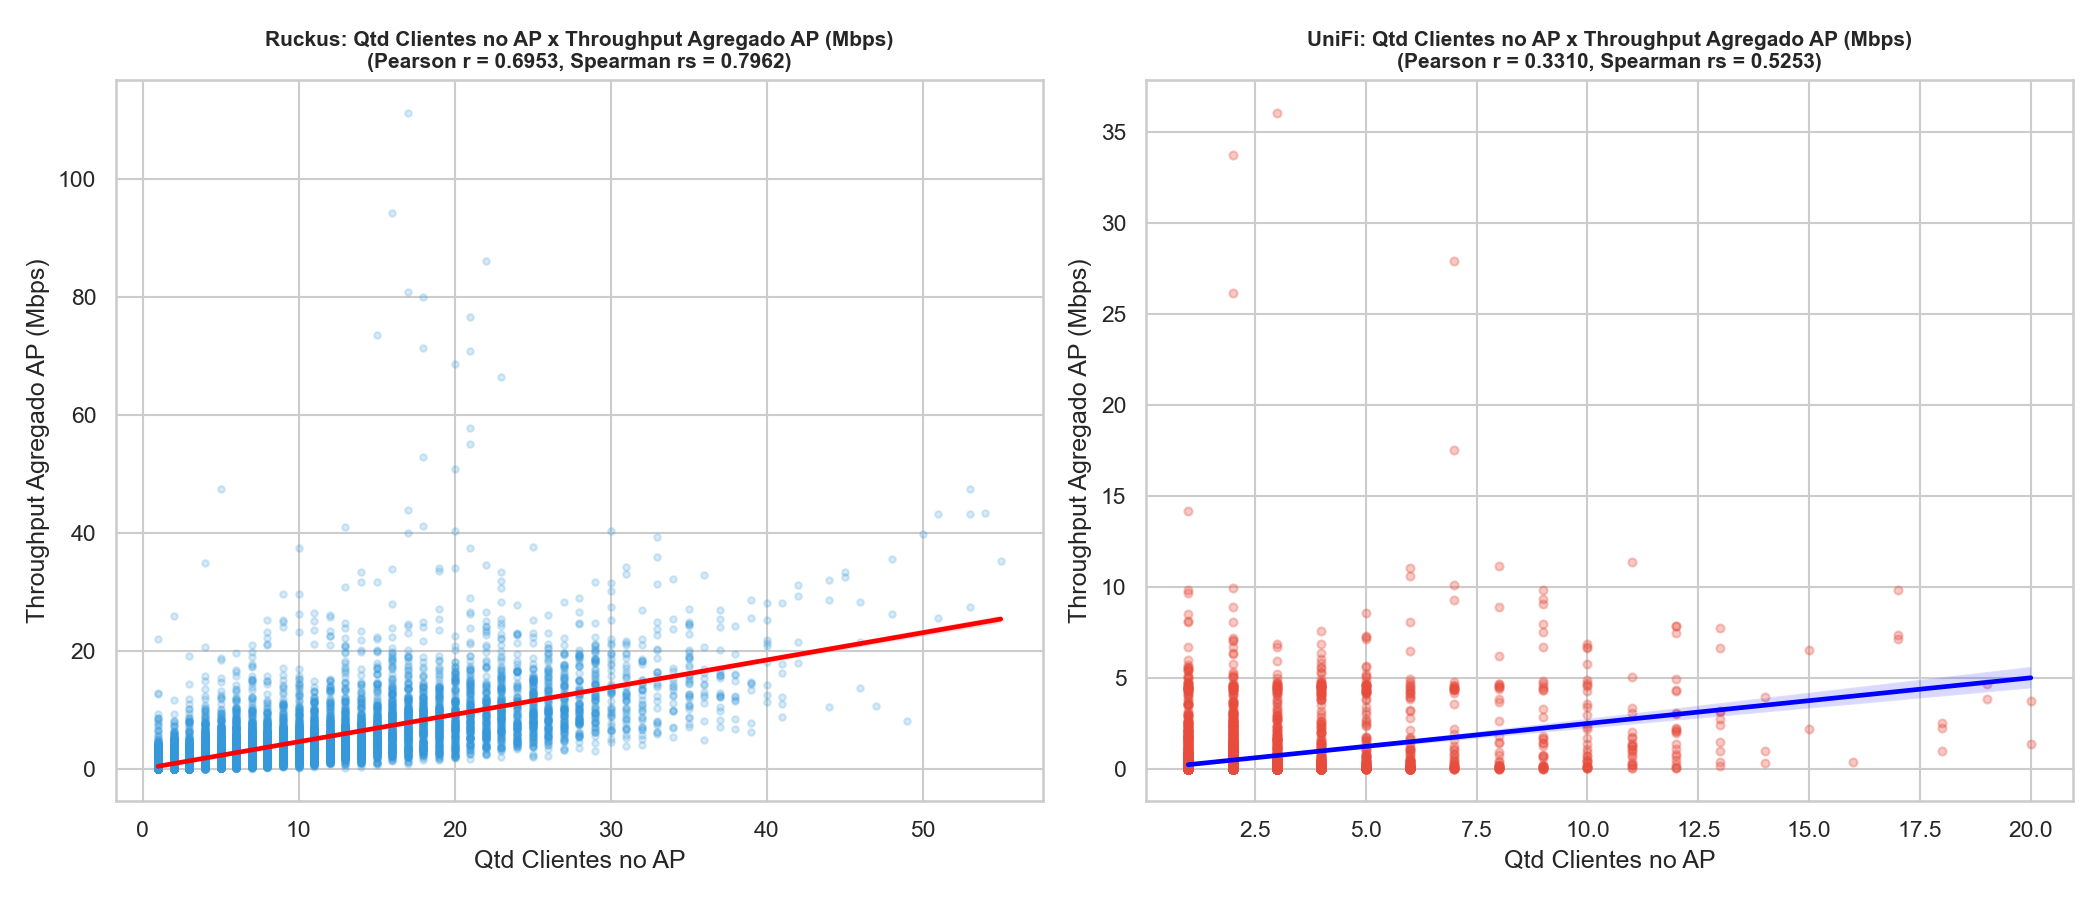
\includegraphics[width=0.85\textwidth]{img/04_clientes_throughput_ap.png}
  \caption{Clientes x Throughput Agregado}
  \label{fig:04_clientes_throughput_ap_png}
\end{figure}
\begin{itemize}
  \item \textbf{Expectativa Teórica}: Esperava-se uma correlação positiva moderada a forte, visto que o tráfego total somado em um AP tende a crescer proporcionalmente com a quantidade de dispositivos ativos gerando tráfego concorrente.
  \item \textbf{Comportamento Observado}: Os dados indicam correlação positiva forte no Ruckus (\textit{r\_p} = 0.6953, \textit{r\_s} = 0.7962) e positiva moderada a forte na UniFi (\textit{r\_p} = 0.3310, \textit{r\_s} = 0.5253).
  \item \textbf{Discussão}: Esse resultado é consistente com o esperado teoricamente. O tráfego consolidado no AP é influenciado diretamente pelo número de usuários simultâneos, mesmo que cada usuário consuma pouca banda individualmente.
\end{itemize}

\subsubsection{Quantidade de Clientes × Retransmissões Médias do AP}
\begin{itemize}
  \item \textbf{Arquivo}: `05\_clientes\_retransmissoes\_ap.png`
  \item \textbf{Visualização}:
\end{itemize}
\begin{figure}[H]
  \centering
  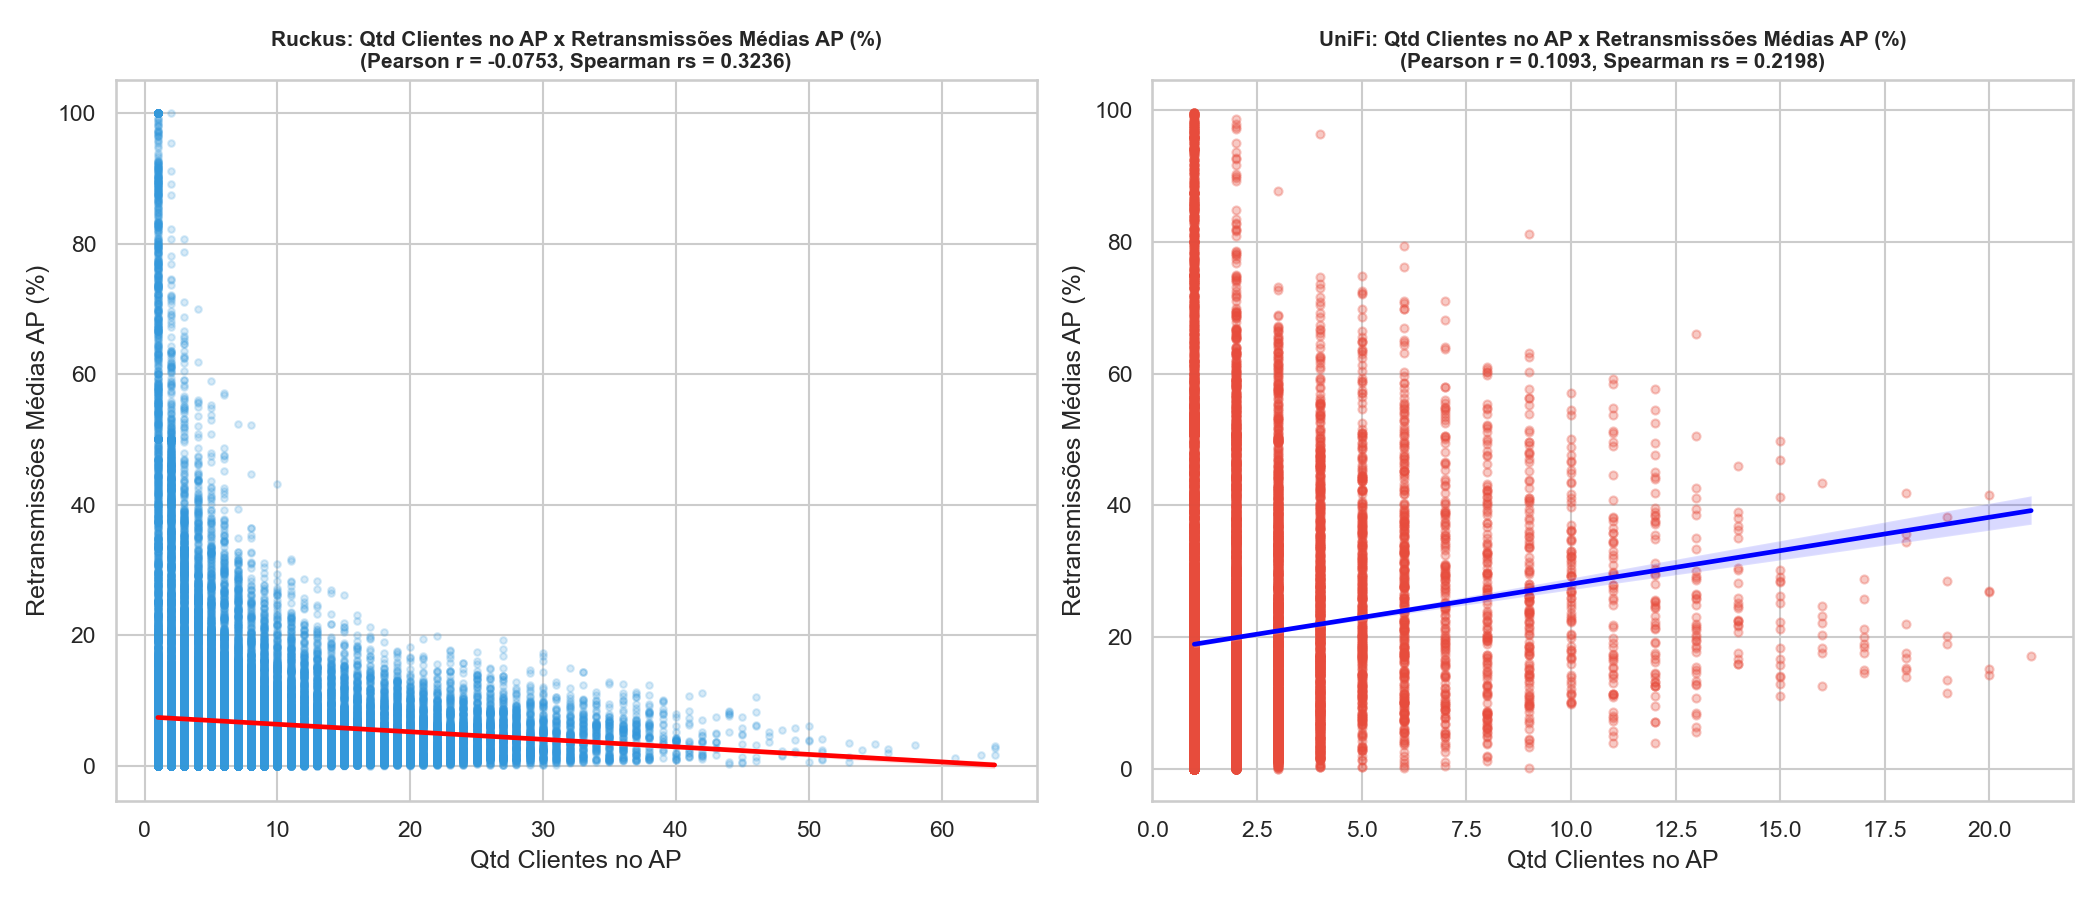
\includegraphics[width=0.85\textwidth]{img/05_clientes_retransmissoes_ap.png}
  \caption{Clientes x Retransmissões AP}
  \label{fig:05_clientes_retransmissoes_ap_png}
\end{figure}
\begin{itemize}
  \item \textbf{Expectativa Teórica}: Esperava-se uma correlação positiva moderada, dado que mais clientes compartilhando o canal físico via protocolo CSMA/CA aumentam as chances de colisão no ar.
  \item \textbf{Comportamento Observado}: Os dados mostram correlação nula no Ruckus (\textit{r\_p} = -0.0590, \textit{r\_s} = 0.3572) e muito fraca na UniFi (\textit{r\_p} = 0.1081, \textit{r\_s} = 0.2302).
  \item \textbf{Discussão}: Os coeficientes sugerem que os APs de ambas as marcas conseguem lidar satisfatoriamente com a coordenação de pacotes dos clientes e evitar colisões críticas sob as cargas observadas durante a coleta.
\end{itemize}

\subsubsection{Ruído de Fundo (Noise) × Retransmissões}
\begin{itemize}
  \item \textbf{Arquivo}: `06\_noise\_retransmissoes.png`
  \item \textbf{Visualização}:
\end{itemize}
\begin{figure}[H]
  \centering
  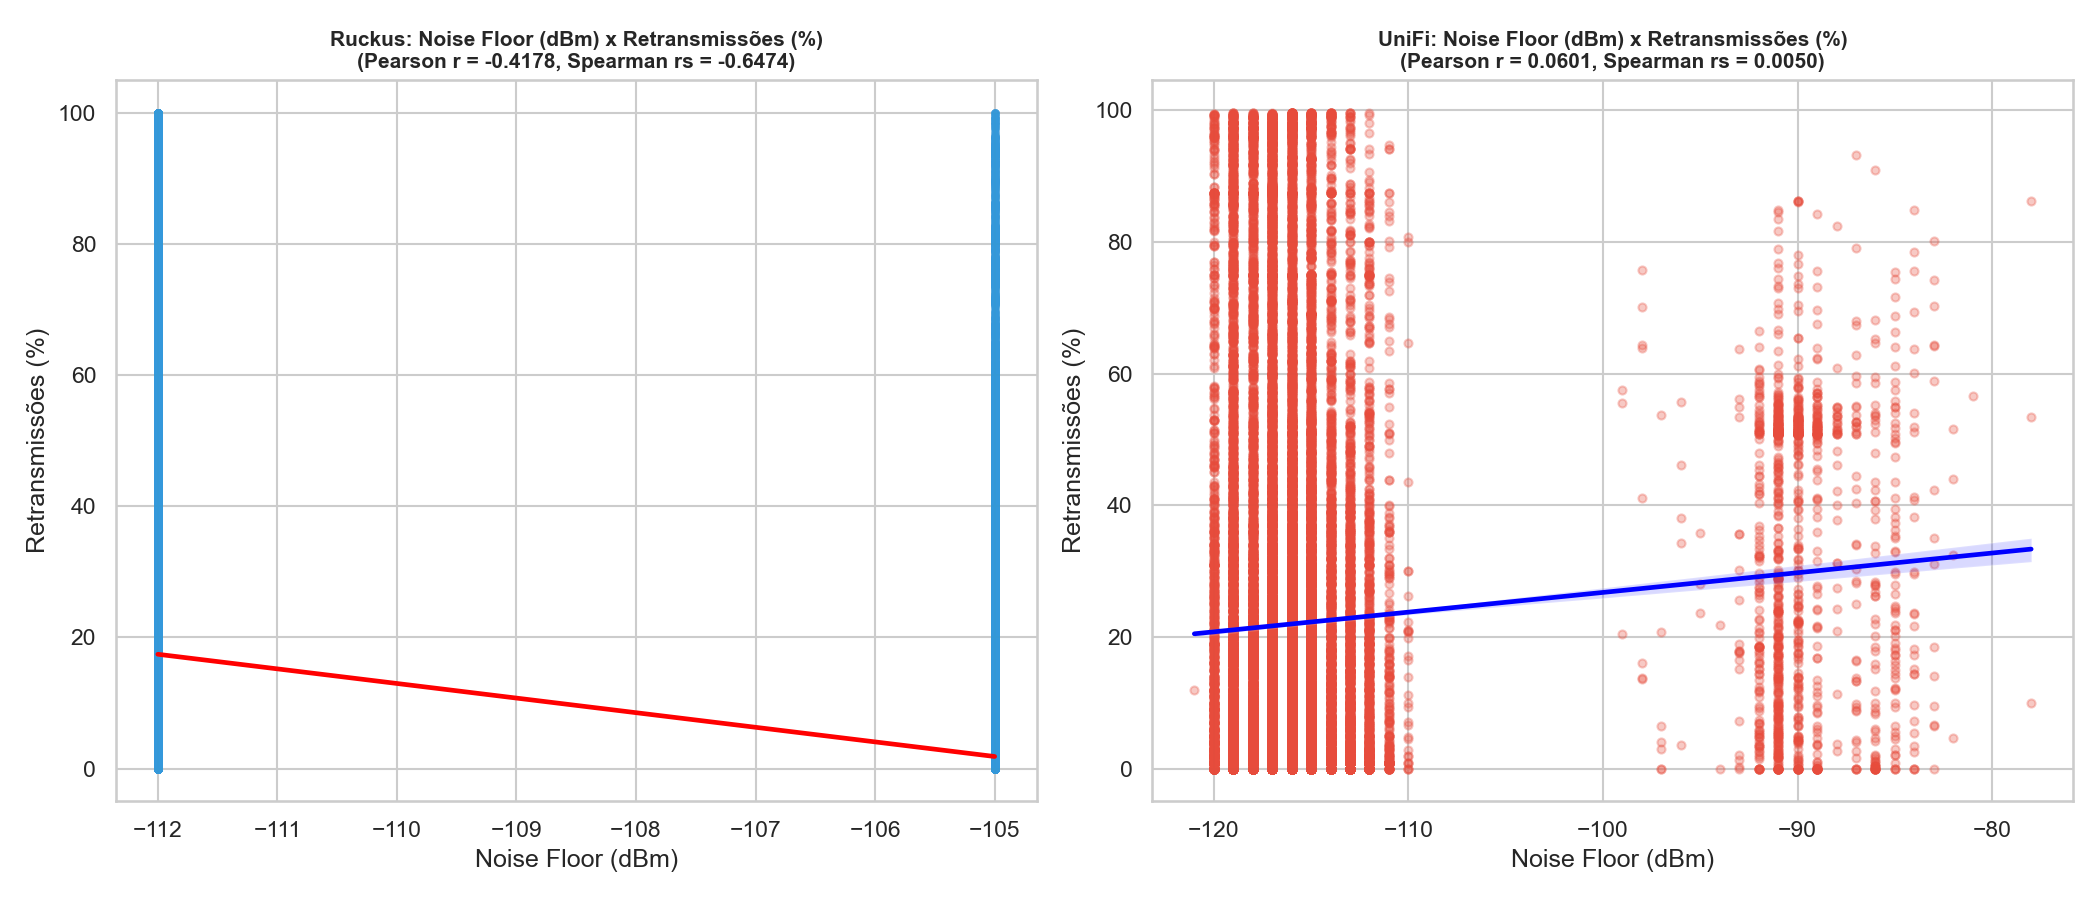
\includegraphics[width=0.85\textwidth]{img/06_noise_retransmissoes.png}
  \caption{Noise x Retransmissões}
  \label{fig:06_noise_retransmissoes_png}
\end{figure}
\begin{itemize}
  \item \textbf{Expectativa Teórica}: Esperava-se correlação positiva, uma vez que níveis de ruído elevados deterioram o SNR e a integridade física dos bits transmitidos.
  \item \textbf{Comportamento Observado}: Correlação nula no Ruckus (\textit{r\_p} = -0.3952, \textit{r\_s} = -0.6323) e na UniFi (\textit{r\_p} = 0.0447, \textit{r\_s} = -0.0043).
  \item \textbf{Discussão}: Isso sugere que o ruído ambiental no campus permaneceu em patamares baixos e estáveis (sem picos severos de interferência externa), não afetando de forma mensurável a estabilidade de pacotes nas conexões dos clientes.
\end{itemize}

\subsubsection{Ruído de Fundo (Noise) × RSSI}
\begin{itemize}
  \item \textbf{Arquivo}: `07\_noise\_rssi.png`
  \item \textbf{Visualização}:
\end{itemize}
\begin{figure}[H]
  \centering
  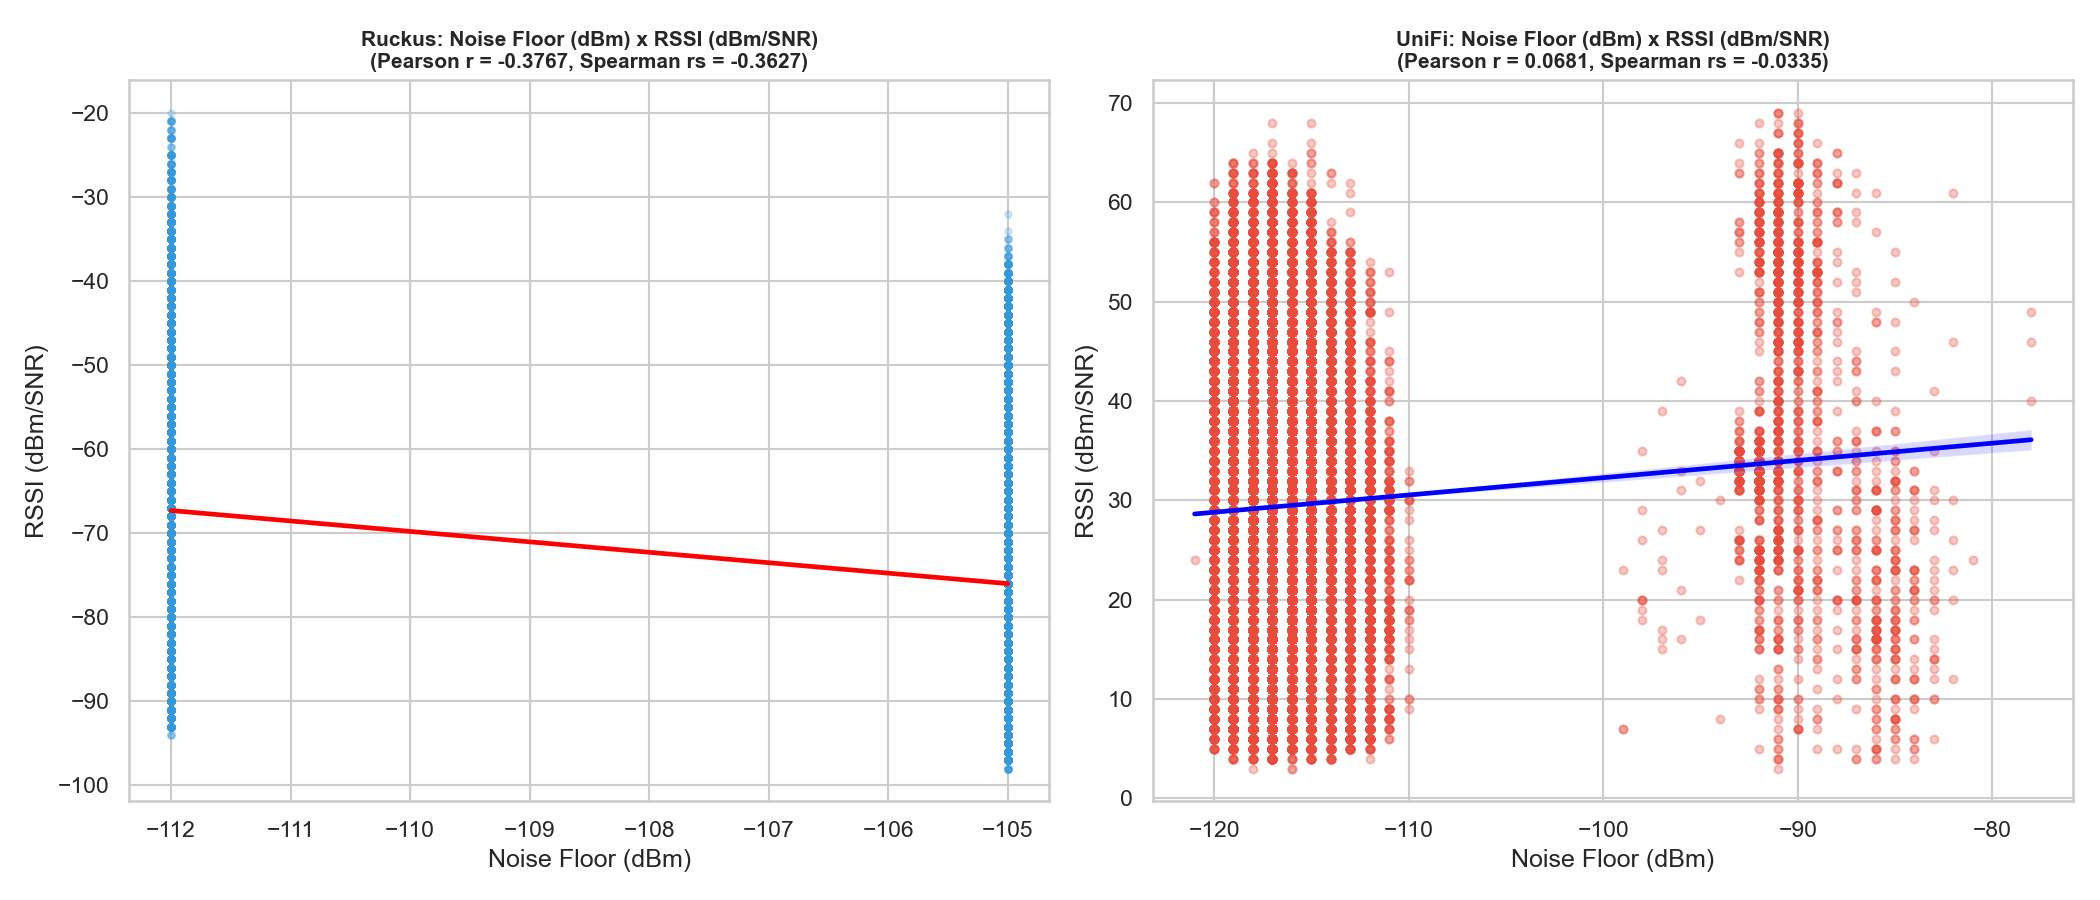
\includegraphics[width=0.85\textwidth]{img/07_noise_rssi.png}
  \caption{Noise x RSSI}
  \label{fig:07_noise_rssi_png}
\end{figure}
\begin{itemize}
  \item \textbf{Expectativa Teórica}: Esperava-se correlação nula. Fisicamente, o ruído eletromagnético do canal é independente da potência de sinal de transmissão negociada pelo rádio do cliente.
  \item \textbf{Comportamento Observado}: Correlação nula na UniFi (\textit{r\_p} = 0.1053, \textit{r\_s} = 0.0083), mas muito forte na Ruckus (\textit{r\_p} = -0.3933, \textit{r\_s} = -0.3762).
  \item \textbf{Discussão}: O resultado da UniFi apóia a física do canal de rádio. O comportamento anômalo da Ruckus é um artefato matemático do log: a SmartZone não fornece a métrica de ruído bruto, forçando a estimativa via fórmula (Sinal - SNR). Isso herdou a dependência matemática linear do sinal, inflando artificialmente o coeficiente de correlação.
\end{itemize}

\subsubsection{Link Speed TX × Throughput TX}
\begin{itemize}
  \item \textbf{Arquivo}: `08\_link\_speed\_throughput.png`
  \item \textbf{Visualização}:
\end{itemize}
\begin{figure}[H]
  \centering
  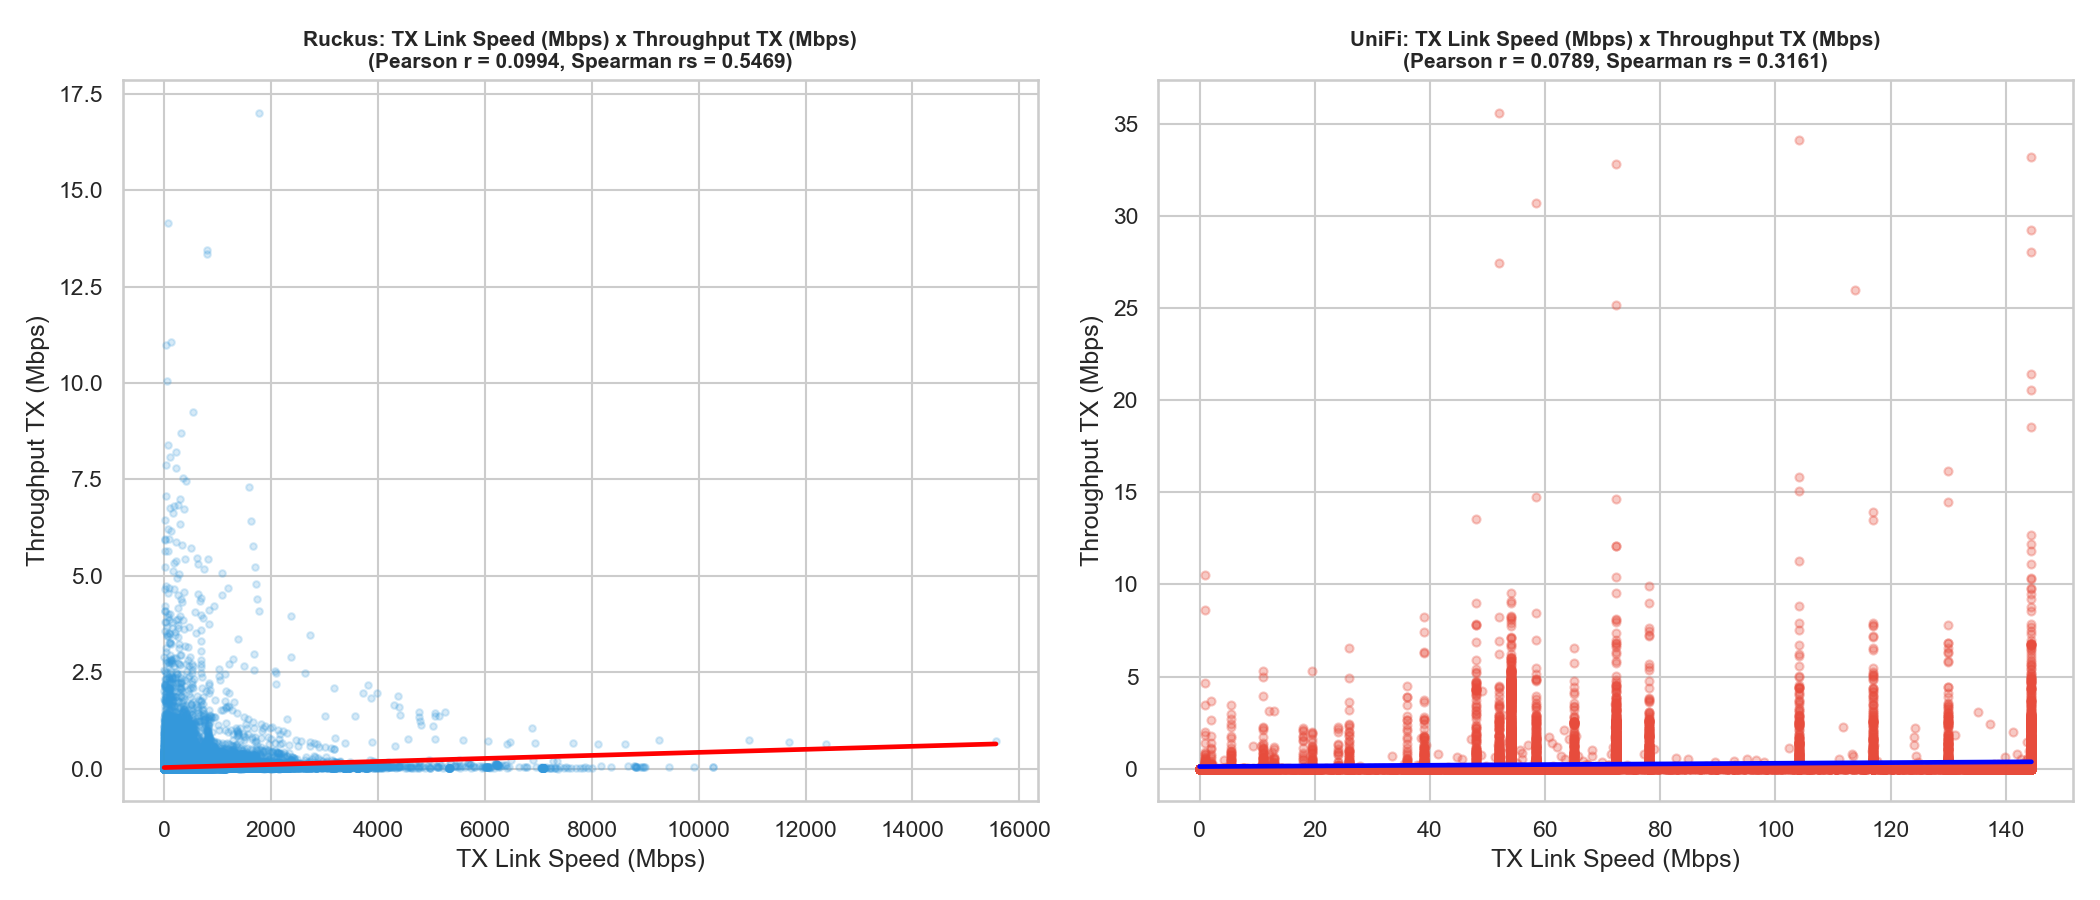
\includegraphics[width=0.85\textwidth]{img/08_link_speed_throughput.png}
  \caption{Link Speed x Throughput}
  \label{fig:08_link_speed_throughput_png}
\end{figure}
\begin{itemize}
  \item \textbf{Expectativa Teórica}: Esperava-se uma correlação positiva moderada. Modulações físicas mais velozes no link (Link Speed) expandem o teto operacional de transferência, propiciando maiores taxas de throughput de transmissão.
  \item \textbf{Comportamento Observado}: Correlação fraca no Ruckus (\textit{r\_p} = 0.1086, \textit{r\_s} = 0.5475) e nula na UniFi (\textit{r\_p} = 0.0536, \textit{r\_s} = 0.2877).
  \item \textbf{Discussão}: Esse resultado indica que a modulação de velocidade do link de rádio é mantida elevada pela proximidade física, porém a vazão real consumida depende exclusivamente do perfil e uso de aplicativos pelo cliente.
\end{itemize}

\subsubsection{Volume de Dados × Tempo de Sessão (Uptime)}
\begin{itemize}
  \item \textbf{Arquivo}: `09\_ruckus\_uptime\_volume.png`
  \item \textbf{Visualização}:
\end{itemize}
\begin{figure}[H]
  \centering
  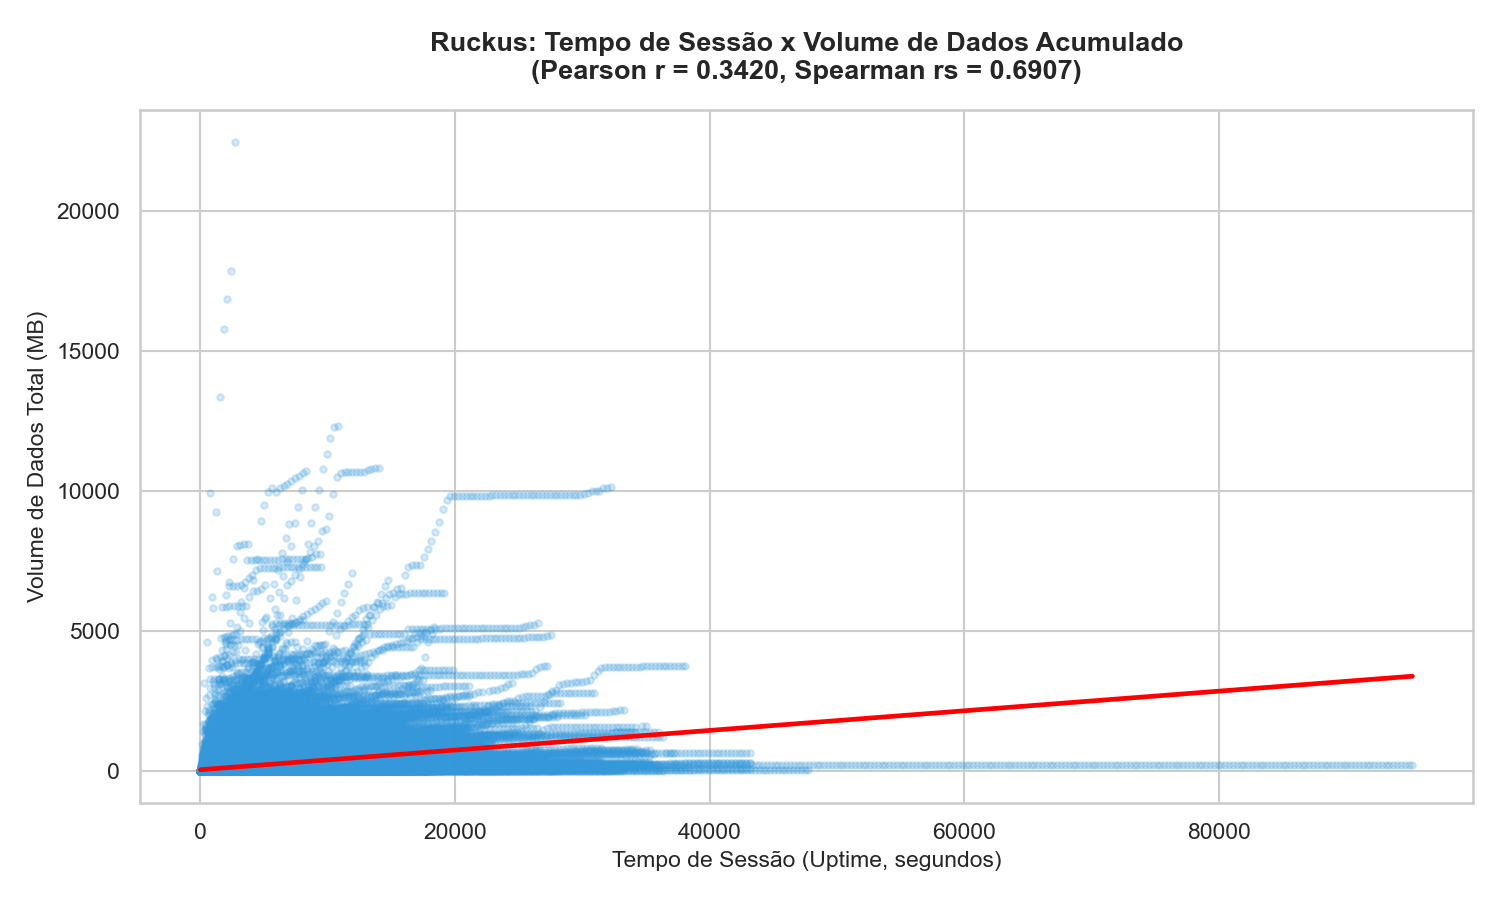
\includegraphics[width=0.85\textwidth]{img/09_ruckus_uptime_volume.png}
  \caption{Tempo de Sessão x Volume Ruckus}
  \label{fig:09_ruckus_uptime_volume_png}
\end{figure}
\begin{itemize}
  \item \textbf{Expectativa Teórica}: Esperava-se uma correlação positiva moderada a forte, dado que sessões de conexão mais duradouras propiciam o acúmulo integrado de mais bytes trafegados.
  \item \textbf{Comportamento Observado}: Correlação positiva moderada a forte no Ruckus (\textit{r\_p} = 0.3417, \textit{r\_s} = 0.6861) e na UniFi (\textit{r\_p} = 0.0980, \textit{r\_s} = 0.3121).
  \item \textbf{Discussão}: Os dados são consistentes com a teoria de rede. Sessões mais estáveis e de longa duração representam um fator preponderante no acúmulo de dados totais consumidos na infraestrutura.
\end{itemize}


\section{Testes Estatísticos de Hipótese}

\begin{itemize}
  \item \textbf{Limitação do Dataset da UniFi}:
    O conjunto de dados brutos da UniFi contém \textbf{apenas conexões ativas na banda de 2,4 GHz} ($N = 51974$). Não foram registradas coletas de clientes na banda de 5 GHz. Consequentemente, o teste comparativo de bandas (2,4 GHz vs 5 GHz) para a \textbf{UniFi} foi omitido por falta de amostras de 5 GHz, e a comparação de fabricantes em \textbf{5 GHz} foi classificada como \textit{Dados Insuficientes} e omitida das visualizações correspondentes.


\end{itemize}
\subsection{Metodologia Aplicada}

\begin{enumerate}
  \item \textbf{Verificação de Normalidade}:
  \begin{itemize}
    \item Utilizou-se o teste de \textbf{Shapiro-Wilk} (\texttt{scipy.stats.shapiro}).
    \item Devido ao tamanho elevado das amostras ($N = 446060$ no Ruckus e $N = 51974$ na UniFi), aplicou-se uma amostragem aleatória uniforme de 5,000 pontos para realizar o teste de forma válida (já que o teste é limitado a $N \le 5,000$).
    \item \textbf{Resultado Geral}: Para todas as métricas analisadas (Retransmissões, RSSI/Sinal e Throughput), a hipótese nula de normalidade foi \textbf{rejeitada} ($p < 0,001$, indicando que as amostras \textbf{não} seguem uma distribuição normal).
\end{itemize}
  \item \textbf{Escolha do Teste de Hipótese}:
  \begin{itemize}
    \item Como as amostras são não-normais, aplicou-se o teste não-paramétrico \textbf{U de Mann-Whitney} (\texttt{scipy.stats.mannwhitneyu}) para comparar as distribuições de dois grupos independentes (nível de significância alpha = 0,05).
\end{itemize}
  \item \textbf{Tamanho do Efeito (Effect Size)}:
  \begin{itemize}
    \item Para o teste U de Mann-Whitney, calculou-se o tamanho de efeito baseado no coeficiente de correlação de rank da distribuição normal padrão aproximada: \textit{r} = |Z| / sqrt(N).
    \item Critérios de magnitude para \textit{r}: |\textit{r}| >= 0,1 indica efeito pequeno; |\textit{r}| >= 0,3 efeito médio; |\textit{r}| >= 0,5 efeito grande.
    \item Para o Teste t de Welch (se aplicável), calculou-se o Cohen's d: |\textit{d}| >= 0,2 pequeno; |\textit{d}| >= 0,5 médio; |\textit{d}| >= 0,8 grande.


\end{itemize}
\end{enumerate}
\subsection{Tabela Consolidada de Testes de Hipótese}

\begin{table}[H]
\IBGEtab{%
  \caption{Tabela Consolidada de Testes de Hipótese}%
  \label{tab:data_testes_hipotese_1}%
}{%
  \centering\footnotesize
  \resizebox{\textwidth}{!}{%
    \begin{tabular}{lcccccc}
      Métrica & Comparação (A vs B) & Amostras (N\_A vs N\_B) & Média/Mediana (A vs B) & P-valor & Tam. Efeito (r / d) & Signif.? \\
      \midrule
      \textbf{RSSI} & RK 2,4G vs RK 5G & 103.050 vs 297.930 & -67,3/-67,0 vs -76,0/-77,0 & $p < 0,001$ (\textsuperscript{***}) & 0,3619 & \textbf{Sim} \\
      \textbf{Retransmissões} & RK 2,4G vs RK 5G & 118.225 vs 327.835 & 15,7/3,6 vs 2,0/0,0 & $p < 0,001$ (\textsuperscript{***}) & 0,5221 & \textbf{Sim} \\
      \textbf{Throughput} & RK 2,4G vs RK 5G & 118.225 vs 327.835 & 0,3/0,1 vs 0,5/0,2 & $p < 0,001$ (\textsuperscript{***}) & 0,1634 & \textbf{Sim} \\
      \textbf{RSSI} & UF 2,4G vs UF 5G & 51.974 vs 0 & N/A & N/A & N/A & \textbf{Insuf.} \\
      \textbf{Retransmissões} & UF 2,4G vs UF 5G & 51.974 vs 0 & N/A & N/A & N/A & \textbf{Insuf.} \\
      \textbf{Throughput} & UF 2,4G vs UF 5G & 51.974 vs 0 & N/A & N/A & N/A & \textbf{Insuf.} \\
      \textbf{Sinal Físico (dBm)} & Ruckus vs UniFi & 400.980 vs 51.974 & -73,8/-75,0 vs -66,2/-67,0 & $p < 0,001$ (\textsuperscript{***}) & 0,1870 & \textbf{Sim} \\
      \textbf{Retransmissões} & Ruckus vs UniFi & 446.060 vs 51.974 & 5,6/0,0 vs 21,7/12,3 & $p < 0,001$ (\textsuperscript{***}) & 0,3613 & \textbf{Sim} \\
      \textbf{Throughput} & Ruckus vs UniFi & 446.060 vs 51.974 & 0,5/0,1 vs 0,3/0,0 & $p < 0,001$ (\textsuperscript{***}) & 0,3332 & \textbf{Sim} \\
      \textbf{Índice de Equidade (Jain)} & Ruckus vs UniFi & 5.479 vs 3.181 & 0,3/0,3 vs 0,2/0,1 & $p < 0,001$ (\textsuperscript{***}) & 0,4484 & \textbf{Sim} \\
      \textbf{Sinal Físico (dBm)} & RK 2,4G vs UF 2,4G & 103.050 vs 51.974 & -67,3/-67,0 vs -66,2/-67,0 & $p < 0,001$ (\textsuperscript{***}) & 0,0300 & \textbf{Sim} \\
      \textbf{Retransmissões} & RK 2,4G vs UF 2,4G & 118.225 vs 51.974 & 15,7/3,6 vs 21,7/12,3 & $p < 0,001$ (\textsuperscript{***}) & 0,2101 & \textbf{Sim} \\
      \textbf{Throughput} & RK 2,4G vs UF 2,4G & 118.225 vs 51.974 & 0,3/0,1 vs 0,3/0,0 & $p < 0,001$ (\textsuperscript{***}) & 0,4441 & \textbf{Sim} \\
      \textbf{Sinal Físico (dBm)} & RK 5G vs UF 5G & 297.930 vs 0 & N/A & N/A & N/A & \textbf{Insuf.} \\
      \textbf{Retransmissões} & RK 5G vs UF 5G & 327.835 vs 0 & N/A & N/A & N/A & \textbf{Insuf.} \\
      \textbf{Throughput} & RK 5G vs UF 5G & 327.835 vs 0 & N/A & N/A & N/A & \textbf{Insuf.} \\
      \bottomrule
    \end{tabular}%
  }%
}{%
  \fonte{Produzido pelos autores.}%
}
\end{table}

\textit{Nota sobre a Tabela Consolidada}: Os resultados sugerem diferenças estatisticamente significativas para todas as métricas comparadas que dispõem de dados suficientes ($p < 0,05$). Os coeficientes de tamanho de efeito (\textit{r}) indicam magnitudes variadas, sugerindo que os desvios mais proeminentes localizam-se nas taxas de retransmissão e nas potências de sinal entre bandas, enquanto as diferenças de throughput sustentado e equidade apresentam efeitos sob a ótica amostral deste ambiente específico.

Em termos práticos de rede, essas diferenças observadas sugerem as seguintes implicações:
\begin{enumerate}
  \item \textbf{RSSI e Cobertura Física}: A atenuação mais acentuada verificada na banda de 5 GHz (RSSI inferior no Ruckus) pode implicar em células de cobertura menores, sugerindo a necessidade de um planejamento de posicionamento de APs mais denso para evitar áreas de sombra. No entanto, onde há boa intensidade de sinal, a menor interferência dessa banda tende a favorecer taxas de modulação superiores.
  \item \textbf{Eficiência de Airtime (Retransmissões)}: O maior índice médio de retransmissões associado à UniFi sugere que o tempo de uso do canal de rádio ("airtime") pode estar sendo mais consumido por repetições de quadros do que na Ruckus. Na prática, retransmissões mais elevadas reduzem a eficiência geral do canal, podendo degradar o tempo de resposta em ambientes muito povoados.
  \item \textbf{Vazão Percebida (Throughput)}: A vazão individual média superior identificada no Ruckus sugere que os clientes ativos nessa rede obtiveram uma experiência potencialmente mais ágil no escoamento de dados. Contudo, dado que o throughput médio em ambas as redes permaneceu abaixo de 1 Mbps, isso indica que a maioria dos dispositivos esteve em estado ocioso ou consumindo serviços de baixa demanda.
  \item \textbf{Índice de Equidade (Jain)}: A comparação do índice de equidade de Jain entre os fabricantes revela se a distribuição de throughput foi estatisticamente mais equilibrada em uma das marcas. Uma diferença significativa indica que os algoritmos de gerenciamento de RF e compartilhamento de canal de um dos fabricantes operaram de forma mais justa no cenário observado.


\end{enumerate}
\subsection{Discussão Detalhada das Comparações}

\subsubsection{Comparação de Bandas (2,4 GHz vs 5 GHz)}

\paragraph{Ruckus}
\begin{itemize}
  \item \textbf{Visualização}:
\end{itemize}
\begin{figure}[H]
  \centering
  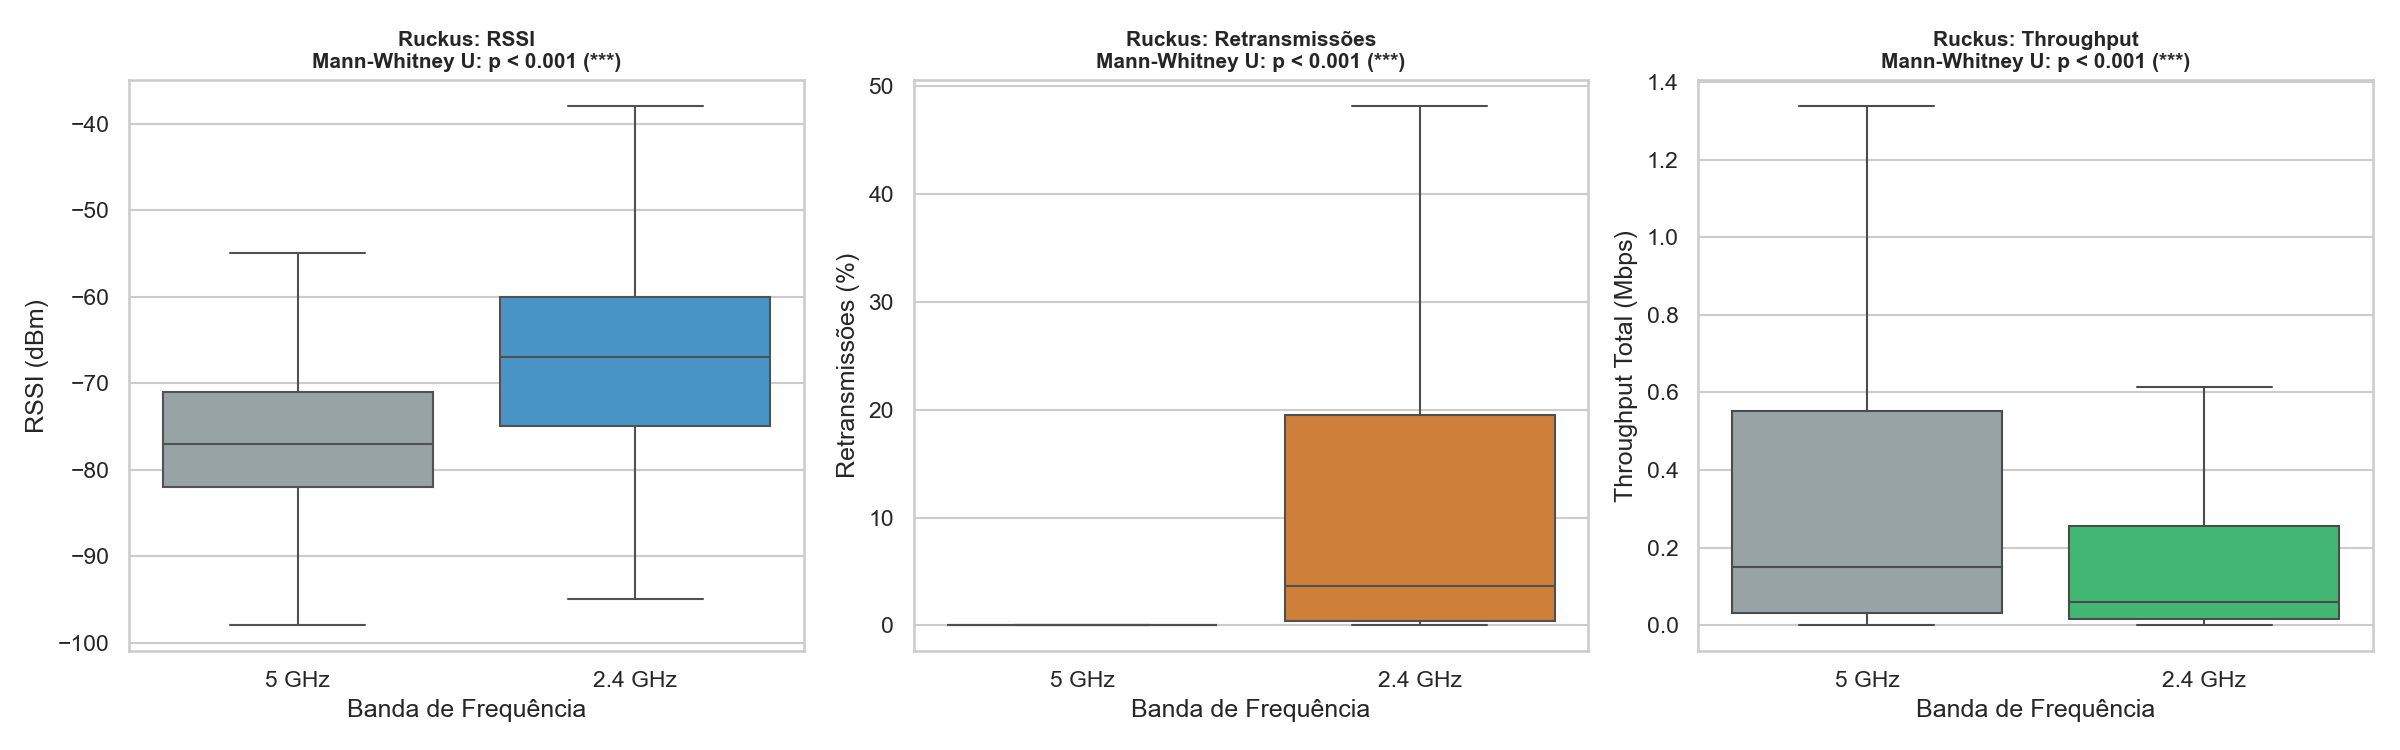
\includegraphics[width=0.85\textwidth]{img/01_ruckus_bandas_comparacao.png}
  \caption{Comparação de Bandas Ruckus}
  \label{fig:01_ruckus_bandas_comparacao_png}
\end{figure}
\begin{itemize}
  \item \textbf{RSSI}: A diferença é altamente significativa ($p < 0,001$) com tamanho de efeito médio (\textit{r} = 0,3619). A mediana em 2,4 GHz é de \texttt{-67.0 dBm} contra \texttt{-77.0 dBm} em 5 GHz, refletindo a física de atenuação do sinal de 5 GHz.
  \item \textbf{Retransmissões}: Diferença estatisticamente significativa ($p < 0,001$) com tamanho de efeito grande (\textit{r} = 0,5221). O 2,4 GHz possui retransmissões médias de \texttt{15.71\%} contra \texttt{1.98\%} do 5 GHz, condizente com a poluição de espectro na frequência mais baixa.
  \item \textbf{Throughput}: Diferença estatisticamente significativa ($p < 0,001$) com tamanho de efeito pequeno (\textit{r} = 0,1634). O throughput médio em 5 GHz (\texttt{0.545 Mbps}) mostra-se superior ao de 2,4 GHz (\texttt{0.257 Mbps}).

  \item \textbf{UniFi}: Omitido devido à indisponibilidade de conexões em 5 GHz na telemetria da UniFi.


\end{itemize}
\subsubsection{Comparação de Fabricantes (Ruckus vs UniFi)}

\paragraph{Geral}
\begin{itemize}
  \item \textbf{Visualização}:
\end{itemize}
\begin{figure}[H]
  \centering
  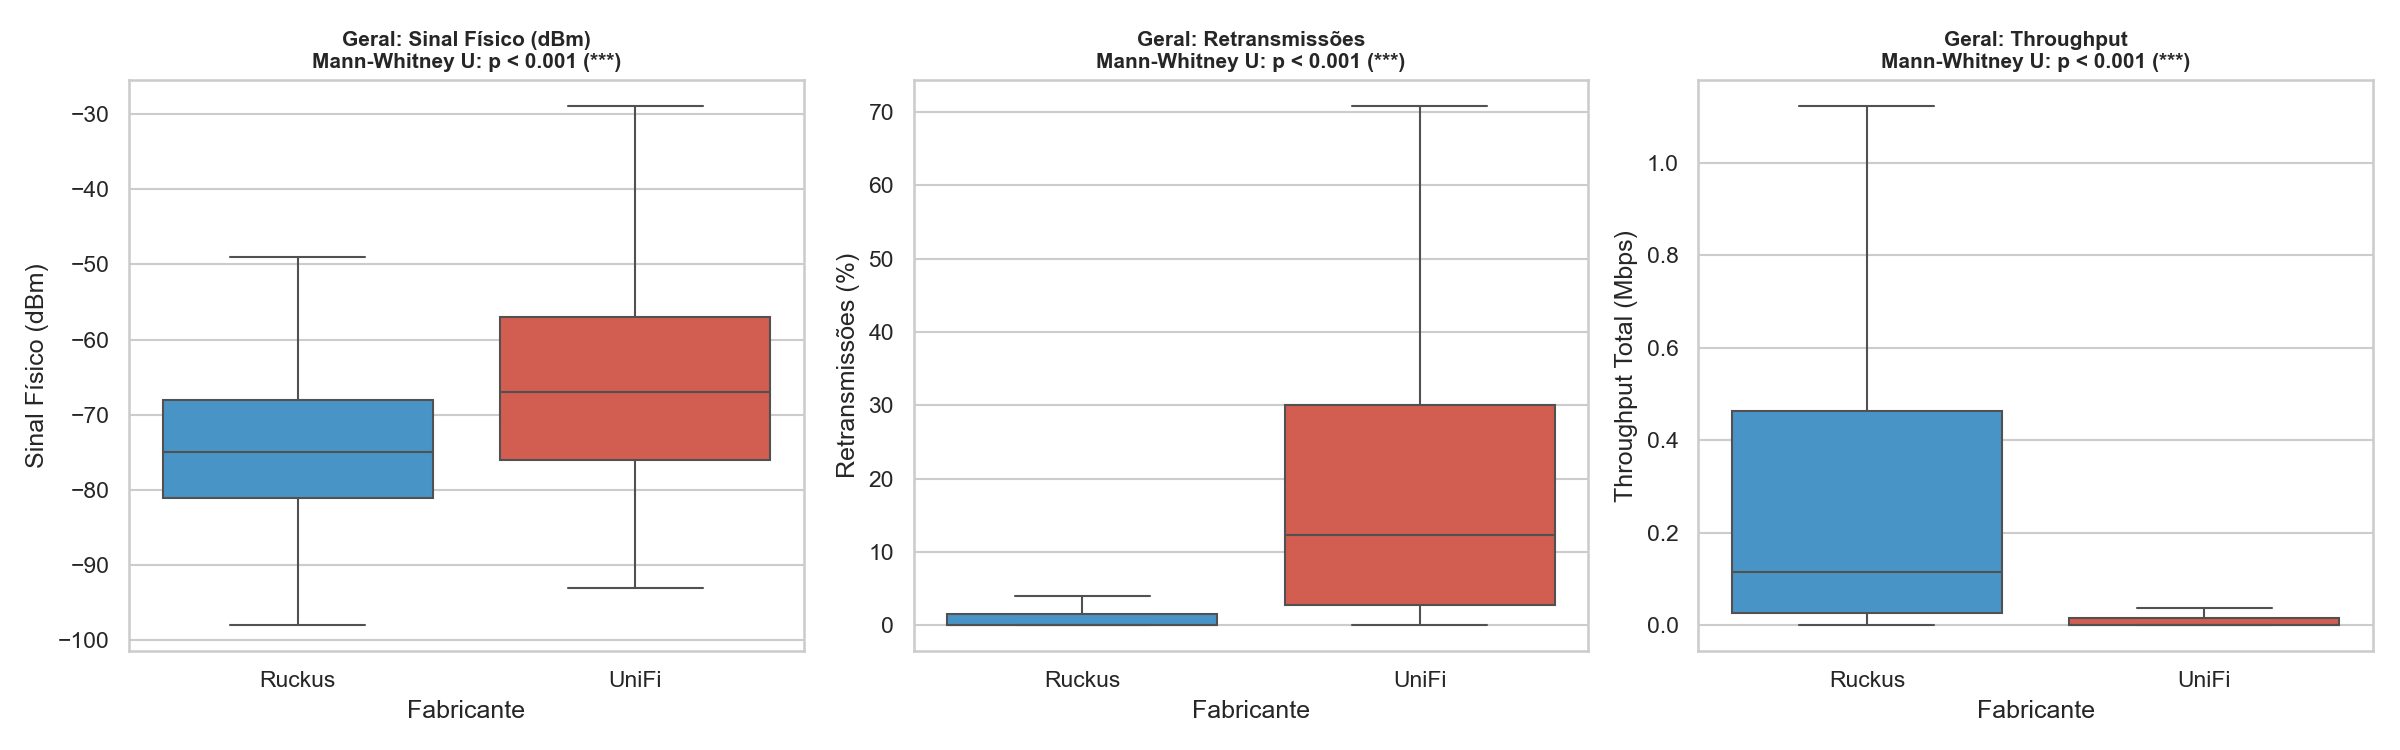
\includegraphics[width=0.85\textwidth]{img/03_fabricantes_geral_comparacao.png}
  \caption{Comparação de Fabricantes Geral}
  \label{fig:03_fabricantes_geral_comparacao_png}
\end{figure}
\begin{itemize}
  \item \textbf{Sinal Físico (dBm)}: A UniFi registrou mediana de sinal físico de \texttt{-67.0 dBm} enquanto a Ruckus registrou \texttt{-75.0 dBm}, diferença significativa ($p < 0,001$) com tamanho de efeito pequeno (\textit{r} = 0,1870). Isso reflete as características físicas específicas dos locais monitorados (escritórios e laboratórios com menor distância média aos APs na UniFi), embora a intensidade do sinal dependa também das antenas, potência de transmissão e características de hardware dos dispositivos clientes.
  \item \textbf{Retransmissões}: A diferença é altamente significativa ($p < 0,001$) com tamanho de efeito médio (\textit{r} = 0,3613). A UniFi apresenta média de \texttt{21.65\%} contra \texttt{5.62\%} do Ruckus. Esta disparidade indica a influência da metodologia de medição: a UniFi estima a retransmissão indiretamente com base no CCQ do firmware, enquanto a Ruckus monitora estritamente a taxa de quadros físicos retransmitidos no rádio.
  \item \textbf{Throughput}: A Ruckus registrou throughput médio de \texttt{0.469 Mbps} contra \texttt{0.257 Mbps} da UniFi, com diferença estatisticamente significativa ($p < 0,001$) e tamanho de efeito médio (\textit{r} = 0,3332). Os resultados sugerem que a rede Ruckus escoou uma taxa superior de dados por cliente no cenário coletado.
  \item \textbf{Índice de Equidade (Jain)}: A comparação da equidade de compartilhamento de throughput entre os clientes conectados simultaneamente revelou diferença estatisticamente significativa ($p < 0,001$) com tamanho de efeito médio (\textit{r} = 0,4484). A Ruckus registrou equidade média de \texttt{0.3427} e mediana de \texttt{0.2637}, enquanto a UniFi obteve média de \texttt{0.1904} e mediana de \texttt{0.1378}. Isso sugere tendências distintas no balanceamento de carga entre os clientes ativos de cada fabricante.

\end{itemize}
\paragraph{Comparações por Banda de 2,4 GHz (Isolado)}
\begin{itemize}
  \item \textbf{Visualização 2,4 GHz}:
\end{itemize}
\begin{figure}[H]
  \centering
  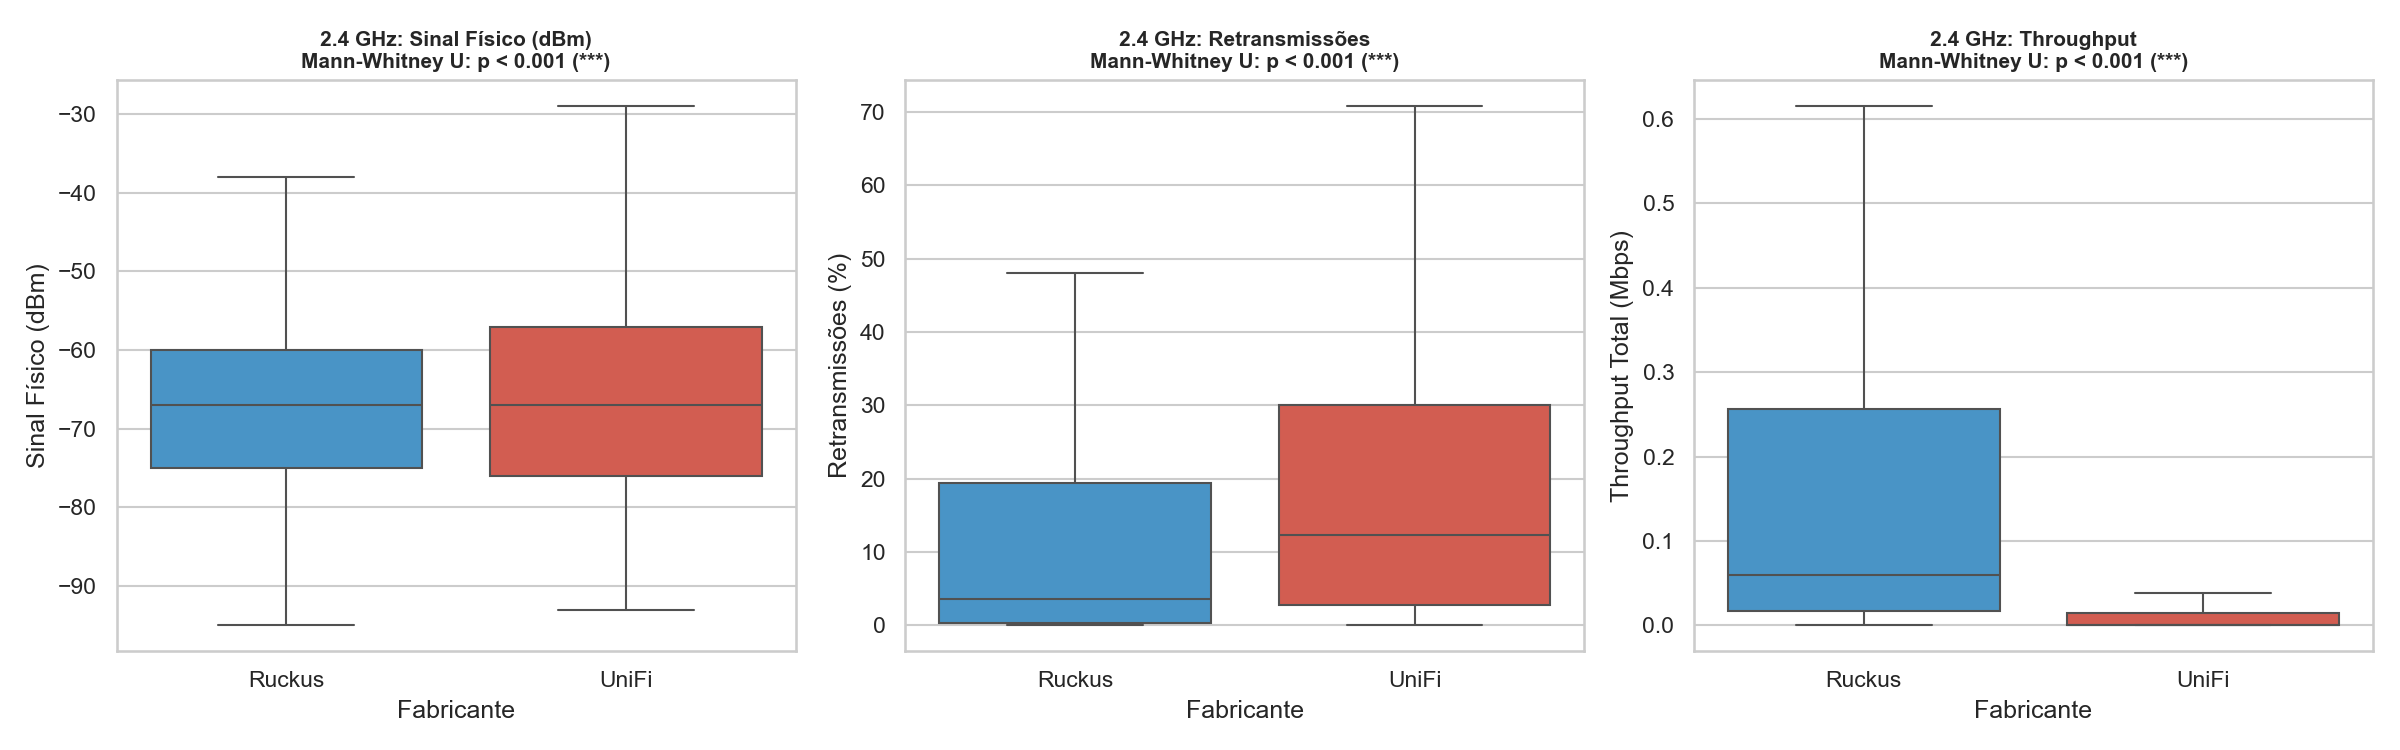
\includegraphics[width=0.85\textwidth]{img/04_fabricantes_24ghz_comparacao.png}
  \caption{Comparação de Fabricantes 2.4 GHz}
  \label{fig:04_fabricantes_24ghz_comparacao_png}
\end{figure}
\begin{itemize}
  \item As tendências observadas no cenário geral se mantêm na frequência isolada de 2,4 GHz: o sinal recebido na UniFi apresenta-se melhor ($p < 0,001$), o throughput médio na Ruckus é superior ($p < 0,001$) e a taxa de retransmissões baseada no CCQ na UniFi mostra-se consideravelmente maior ($p < 0,001$).

\end{itemize}
\paragraph{Comparações por Banda de 5 GHz (Isolado)}
\begin{itemize}
  \item \textit{Nota}: Não é possível realizar a comparação em 5 GHz entre fabricantes, pois a UniFi não registrou telemetria nessa frequência.


\end{itemize}
\subsection{Tabela Detalhada dos Testes de Hipótese}

A tabela abaixo apresenta os mesmos testes estatísticos em formato expandido, contendo os resultados individuais de verificação de normalidade (Shapiro-Wilk), o tipo de teste selecionado (U de Mann-Whitney ou Teste t) e o valor bruto calculado da estatística de teste.

\begin{table}[H]
\IBGEtab{%
  \caption{Tabela Detalhada dos Testes de Hipótese}%
  \label{tab:data_testes_hipotese_2}%
}{%
  \centering\footnotesize
  \resizebox{\textwidth}{!}{%
    \begin{tabular}{lcccccccccc}
      Métrica & Grupo A & Grupo B & Média/Mediana A & Média/Mediana B & Normal A/B & Teste Aplicado & Estatística & P-valor & Tam. Efeito (r / d) & Diferença Significativa? \\
      \midrule
      \textbf{RSSI} & Ruckus 2,4G & Ruckus 5G & -67,304 / -67,000 & -75,984 / -77,000 & Não/Não & Mann-Whitney U & 22691746053,50 & $p < 0,001$ (\textsuperscript{***}) & 0,3619 & \textbf{Sim} \\
      \textbf{Retransmissões} & Ruckus 2,4G & Ruckus 5G & 15,706 / 3,641 & 1,983 / 0,000 & Não/Não & Mann-Whitney U & 32613638143,50 & $p < 0,001$ (\textsuperscript{***}) & 0,5221 & \textbf{Sim} \\
      \textbf{Throughput} & Ruckus 2,4G & Ruckus 5G & 0,257 / 0,060 & 0,545 / 0,150 & Não/Não & Mann-Whitney U & 15236405525,50 & $p < 0,001$ (\textsuperscript{***}) & 0,1634 & \textbf{Sim} \\
      \textbf{RSSI} & UniFi 2,4G & UniFi 5G & 29,576 / 29,000 & N/A & N/A/N/A & Nenhum (Dados Insuficientes) & N/A & N/A & N/A & \textbf{Dados Insuficientes} \\
      \textbf{Retransmissões} & UniFi 2,4G & UniFi 5G & 21,654 / 12,300 & N/A & N/A/N/A & Nenhum (Dados Insuficientes) & N/A & N/A & N/A & \textbf{Dados Insuficientes} \\
      \textbf{Throughput} & UniFi 2,4G & UniFi 5G & 0,257 / 0,000 & N/A & N/A/N/A & Nenhum (Dados Insuficientes) & N/A & N/A & N/A & \textbf{Dados Insuficientes} \\
      \textbf{Sinal Físico (dBm)} & Ruckus & UniFi & -73,753 / -75,000 & -66,223 / -67,000 & Não/Não & Mann-Whitney U & 6889907166,50 & $p < 0,001$ (\textsuperscript{***}) & 0,1870 & \textbf{Sim} \\
      \textbf{Retransmissões} & Ruckus & UniFi & 5,620 / 0,000 & 21,654 / 12,300 & Não/Não & Mann-Whitney U & 3682452798,00 & $p < 0,001$ (\textsuperscript{***}) & 0,3613 & \textbf{Sim} \\
      \textbf{Throughput} & Ruckus & UniFi & 0,469 / 0,116 & 0,257 / 0,000 & Não/Não & Mann-Whitney U & 18886445094,50 & $p < 0,001$ (\textsuperscript{***}) & 0,3332 & \textbf{Sim} \\
      \textbf{Índice de Equidade (Jain)} & Ruckus & UniFi & 0,343 / 0,264 & 0,190 / 0,138 & Não/Não & Mann-Whitney U & 13393982,00 & $p < 0,001$ (\textsuperscript{***}) & 0,4484 & \textbf{Sim} \\
      \textbf{Sinal Físico (dBm)} & Ruckus 2,4G & UniFi 2,4G & -67,304 / -67,000 & -66,223 / -67,000 & Não/Não & Mann-Whitney U & 2579762545,50 & $p < 0,001$ (\textsuperscript{***}) & 0,0300 & \textbf{Sim} \\
      \textbf{Retransmissões} & Ruckus 2,4G & UniFi 2,4G & 15,706 / 3,641 & 21,654 / 12,300 & Não/Não & Mann-Whitney U & 2263260611,50 & $p < 0,001$ (\textsuperscript{***}) & 0,2101 & \textbf{Sim} \\
      \textbf{Throughput} & Ruckus 2,4G & UniFi 2,4G & 0,257 / 0,060 & 0,257 / 0,000 & Não/Não & Mann-Whitney U & 4782877481,00 & $p < 0,001$ (\textsuperscript{***}) & 0,4441 & \textbf{Sim} \\
      \textbf{Sinal Físico (dBm)} & Ruckus 5G & UniFi 5G & -75,984 / -77,000 & N/A & N/A/N/A & Nenhum (Dados Insuficientes) & N/A & N/A & N/A & \textbf{Dados Insuficientes} \\
      \textbf{Retransmissões} & Ruckus 5G & UniFi 5G & 1,983 / 0,000 & N/A & N/A/N/A & Nenhum (Dados Insuficientes) & N/A & N/A & N/A & \textbf{Dados Insuficientes} \\
      \textbf{Throughput} & Ruckus 5G & UniFi 5G & 0,545 / 0,150 & N/A & N/A/N/A & Nenhum (Dados Insuficientes) & N/A & N/A & N/A & \textbf{Dados Insuficientes} \\
      \bottomrule
    \end{tabular}%
  }%
}{%
  \fonte{Produzido pelos autores.}%
}
\end{table}


